% ------------------------------------------------------------------------
% abnTeX2: Modelo de Projeto de pesquisa em conformidade com
% ABNT NBR 15287:2011 Informação e documentação - Projeto de pesquisa -
% Apresentação
% ------------------------------------------------------------------------

\documentclass[
	% -- opções da classe memoir --
	12pt,				% tamanho da fonte
	openright,			% capítulos começam em pág ímpar (insere página vazia caso preciso)
	oneside,			% twoside para impressão em recto e verso. Oposto a oneside
	a4paper,			% tamanho do papel.
	% -- opções da classe abntex2 --
	%chapter=TITLE,		% títulos de capítulos convertidos em letras maiúsculas
	%section=TITLE,		% títulos de seções convertidos em letras maiúsculas
	%subsection=TITLE,	% títulos de subseções convertidos em letras maiúsculas
	%subsubsection=TITLE,% títulos de subsubseções convertidos em letras maiúsculas
	% -- opções do pacote babel --
	english,			% idioma adicional para hifenização
	french,				% idioma adicional para hifenização
	spanish,			% idioma adicional para hifenização
	brazil,				% o último idioma é o principal do documento
	]{abntex2}

% ---
% PACOTES
% ---
% Pacotes fundamentais
% ---
\usepackage{lmodern}			% Usa a fonte Latin Modern
\usepackage[T1]{fontenc}		% Selecao de codigos de fonte.
\usepackage[utf8]{inputenc}		% Codificacao do documento (conversão automática dos acentos)
\usepackage{indentfirst}		% Indenta o primeiro parágrafo de cada seção.
\usepackage{color}				% Controle das cores
\usepackage{graphicx}			% Inclusão de gráficos
\usepackage{microtype} 			% para melhorias de justificação
\usepackage{algpseudocode}
\usepackage{algorithm}
\usepackage{listings}
\usepackage{minted}
\usepackage{tabularx}
% ---
% Pacotes adicionais, usados apenas no âmbito do Modelo Canônico do abnteX2
% ---
\usepackage{lipsum}				% para geração de dummy text
% ---
% Pacotes de citações
% ---
\usepackage[brazilian,hyperpageref]{backref}	 % Paginas com as citações na bibl
\usepackage[alf]{abntex2cite}	% Citações padrão ABNT

% ---
% CONFIGURAÇÕES DE PACOTES
% ---
% Configurações do pacote backref
% Usado sem a opção hyperpageref de backref
\renewcommand{\backrefpagesname}{Citado na(s) página(s):~}
% Texto padrão antes do número das páginas
\renewcommand{\backref}{}
% Define os textos da citação
\renewcommand*{\backrefalt}[4]{
	\ifcase #1 %
		Nenhuma citação no texto.%
	\or
		Citado na página #2.%
	\else
		Citado #1 vezes nas páginas #2.%
	\fi}%
% ---

% ---
% Informações de dados para CAPA e FOLHA DE ROSTO
% ---
\titulo{AutoREST\\Uma Ferramenta de\\Geração Automática de REST APIs}
\autor{Lásaro Curtinaz Dumer\\Marcelo Schmitt Laser}
\local{Porto Alegre, Rio Grande do Sul, Brasil}
\orientador{Eduardo Henrique P. de Arruda}
\data{2017}
\instituicao{%
  Pontifícia Universidade Católica do Rio Grande do Sul -- PUCRS
  \par
  Faculdade de Informática
  \par
  Curso de Bacharelado em Ciência da Computação}
\tipotrabalho{Tese (Doutorado)}
% O preambulo deve conter o tipo do trabalho, o objetivo,
% o nome da instituição e a área de concentração
\preambulo{Relatório Final de Trabalho de Conclusão II, apresentado como  requisito  parcial  para obtenção  do  grau  de  Bacharel  em  Ciência  da Computação na Pontifícia    Universidade    Católica    do    Rio Grande  do  Sul}

% ---

% ---
% Configurações de aparência do PDF final

% alterando o aspecto da cor azul
\definecolor{blue}{RGB}{41,5,195}

% informações do PDF
\makeatletter
\hypersetup{
     	%pagebackref=true,
		pdftitle={\@title},
		pdfauthor={\@author},
    	pdfsubject={\imprimirpreambulo},
	    pdfcreator={LaTeX with abnTeX2},
		pdfkeywords={abnt}{latex}{abntex}{abntex2}{projeto de pesquisa},
		colorlinks=true,       		% false: boxed links; true: colored links
    	linkcolor=blue,          	% color of internal links
    	citecolor=blue,        		% color of links to bibliography
    	filecolor=magenta,      		% color of file links
		urlcolor=blue,
		bookmarksdepth=4
}
\makeatother
% ---

% ---
% Espaçamentos entre linhas e parágrafos
% ---
% O tamanho do parágrafo é dado por:
\setlength{\parindent}{1.3cm}
% Controle do espaçamento entre um parágrafo e outro:
\setlength{\parskip}{0.2cm}  % tente também \onelineskip

% ---
% compila o indice
\makeindex
% ---

% ----
% Início do documento
\begin{document}

% Seleciona o idioma do documento (conforme pacotes do babel)
%\selectlanguage{english}
\selectlanguage{brazil}

% Retira espaço extra obsoleto entre as frases.
\frenchspacing

% ----------------------------------------------------------
% ELEMENTOS PRÉ-TEXTUAIS
% ----------------------------------------------------------
% \pretextual

% ---
% Capa
% ---
\imprimircapa
% ---

% ---
% Folha de rosto
% ---
\imprimirfolhaderosto
% ---

% ---
% NOTA DA ABNT NBR 15287:2011, p. 4:
%  ``Se exigido pela entidade, apresentar os dados curriculares do autor em
%     folha ou página distinta após a folha de rosto.''
% ---

% ---
% inserir lista de ilustrações
% ---
\pdfbookmark[0]{\listfigurename}{lof}
\listoffigures*
\cleardoublepage
% ---

% ---
% inserir lista de tabelas
% ---
\pdfbookmark[0]{\listtablename}{lot}
\listoftables*
\cleardoublepage
% ---

% ---
% inserir lista de abreviaturas e siglas
% ---
\begin{siglas}
  \item[REST] Representational State Transfer
  \item[BNF] Backus-Naur Form
  \item[UML] Unified Modeling Language
  \item[OMG] Object Management Group
  \item[W3C] World Wide Web Consortium
  \item[URI] Uniform Resource Identifier
  \item[CASE] Computer-aided software engineering
  \item[IDE] Integrated Development Environment
  \item[JSON] JavaScript Object Notation
  \item[PUCRS] Pontifícia Universidade Católica do Rio Grande do Sul
  \item[CBSE] Component-Based Software Engineering
  \item[GP] Generative Programming
  \item[SPL] Software Product Line
  \item[MDD] Model-Driven Development
  \item[CRUD] Create, Read, Update, Delete
  \item[SGBD] Sistema Gerenciador de Banco de Dados
  \item[CMR] Configuration Model Reader
  \item[PFIS] Processing-Friendly Intermediate Structure
\end{siglas}
% ---

% ---
% inserir lista de símbolos
% ---
%\begin{simbolos}
%  \item[$ \Gamma $] Letra grega Gama
%  \item[$ \Lambda $] Lambda
%  \item[$ \zeta $] Letra grega minúscula zeta
%  \item[$ \in $] Pertence
%\end{simbolos}
% ---

\chapter*{Agradecimentos}

Primeiramente gostaria de agradecer a Deus, pois sei que tudo vem dele, e o desenvolvimento deste trabalho foi uma tarefa muitas vezes desgastante. Dedico este trabalho para minha familia, por ser a minha base e suporte, em especial à minha esposa, Fernanda Dumer, por todo apoio e compreensão durante este trabalho, a quem sou muito grato e amo muito. Também agradeço a meus pais, por toda educação que me deram, por ser a base d quem sou e ter me ajudado a chegar onde estou hoje.

Uma agradecimento especial à meu colega, Marcelo Laser, por todo aprendizado que tivemos juntos, além da troca de conhecimentos e aprendizado que este trabalho nos proporcionou.


\begin{flushright}
Lásaro Dumer    
\end{flushright}


% ---
% inserir o sumario
% ---
\pdfbookmark[0]{\contentsname}{toc}
\tableofcontents*
\cleardoublepage
% ---


% ----------------------------------------------------------
% ELEMENTOS TEXTUAIS
% ----------------------------------------------------------
\textual

%\chapter*[Introdução]{Introdução}
%\addcontentsline{toc}{chapter}{Introdução}

%\citeonline{abntex2classe}.
%\footnote{\url{http://www.latex-project.org/lppl.txt}}.
%\cite{memoir}. Consulte \citeonline{abntex2modelo} para obter

%\index{elementos textuais}A norma ABNT NBR 15287:2011, p. 5, apresenta a

%\begin{citacao}
%O texto deve ser constituído de uma parte introdutória, na qual devem ser
%\end{citacao}

\chapter{Introdução}

Uma das principais preocupações da Engenharia de Software atualmente é a confiabilidade de sistemas e processos de desenvolvimento de software \cite{ROSS:1975} \cite{SOMMERVILLE:2011}. Definida como a prevenção de falhas na concepção, projeto e construção de software, além da capacidade de recuperação de falhas em operação e performance, a confiabilidade de sistemas é dita por Ross como uma preocupação "tardia"\ da Engenharia de Software, muitas vezes ignorada em favor de eficiência.

\citeonline{LYU:1996} apresenta diversas razões para esta preocupação, dentre elas o crescimento dramático do tamanho e complexidade de sistemas computacionais e a forma como sistemas computacionais permeiam quase todas as áreas da sociedade. Como forma de medir a confiabilidade de sistemas, diversos autores \cite{LYU:1996}\cite{MUSA:1979}\cite{REUSSNER:2003} utilizam o quantificar \textit{Mean Time to Failure} (MTTF), ou tempo médio até falha em português. Esta medida é, em todos os casos citados acima, realizada através do teste de software.

Independentemente das abordagens utilizadas, duas técnicas se destacam nos trabalhos de inúmeros autores \cite{JIFENG:2005}\cite{SELIC:2003}\cite{CZARNECKI:2000}\cite{STAHL:2006}\cite{CRNKOVIC:2002a}\cite{CLEMENTS:2001} como uma forma de diminuir consideravelmente o esforço de desenvolvimento e aumentar a confiabilidade de sistemas de software: o reuso de componentes de software testados e maduros, e; a geração automática de código a partir de modelos conceituais.

\citeonline{SELIC:2003} apresenta preocupação sobre o quão atrasada é a Engenharia de Software em buscar melhoras na confiabilidade e produtividade de software. O autor propõe a geração de código automática, a partir de modelos conceituais, como sendo uma mudança fundamental nos paradigmas de desenvolvimento de software, com o potencial de alterar a Engenharia de Software de formas que não são vistas desde a invenção de compiladores, a mais de cinquenta anos.

Já \citeonline{JIFENG:2005} citam dentre as regras de restrição de um componente de software a composição por componentes de terceiros, ressaltando a importância da utilização de componentes de software maduros e testados na composição de sistemas confiáveis. \citeonline{CZARNECKI:2000} e \citeonline{CLEMENTS:2001} reforçam ainda mais a necessidade da criação de grupos de componentes em comum para que a evolução de cada componente seja propagada dentre diversos sistemas.

Os autores citados propõe várias abordagens e tecnologias para a prática dos conceitos propostos nas áreas de geração automática de código e reuso de componentes de software, dentre as quais se destacam neste estudo a Engenharia de Software Baseada em Componentes (CBSE - Component-Based Software Engineering) \cite{CRNKOVIC:2002a}, Programação Generativa (GP - Generative Programming) \cite{CZARNECKI:2000} e o Desenvolvimento Dirigido por Modelos (MDD - Model-Driven Development) \cite{STAHL:2006}.

CBSE se destaca pela identificação de características de software e sua implementação na forma de componentes reutilizáveis, possibilitando a geração de sistemas a partir da composição por partes já mais maduras e confiáveis do que a construção de um sistema inteiramente novo \cite{CRNKOVIC:2002a}. \citeonline{BREIVOLD:2007} citam a facilidade de manutenção de sistemas complexos baseados em CBSE e seu alto grau de uso em sistemas Web, e \citeonline{CRNKOVIC:2000} mencionam que o grau de reuso possibilitado por práticas de CBSE varia desde o reuso de grandes componentes englobando diversas funcionalidades, até o reuso de pequenos blocos de código.

MDD se destaca pelo seu foco em uma documentação minuciosa de um produto de software, tendo a implementação em segundo plano, preferencialmente de forma automatizada, buscando permitir melhor visualização e manutenção do produto \cite{STAHL:2006}. \citeonline{TAYLOR:2009} citam a importância de uma documentação completa de sistemas de software, possibilitando o reuso de partes de sistemas ou até sistemas inteiros em vista do alto grau de compreensão de desenvolvedores que é obtido através do foco em documentação.

GP busca minimizar os trabalhos de programação através da automação de geração de código, realizada pela identificação e formalização das características comuns entre sistemas e a criação de geradores de componentes que os compõe a partir de subcomponentes pré-determinados \cite{CZARNECKI:2000}. \citeonline{BATORY:2004} menciona a abordagem GP como sendo o futuro da engenharia de software, ressaltando a importância de abordagens abrangentes para a geração de sistemas ao invés do uso de soluções \textit{ad hoc}.

O estudo das abordagens de MDD e GP, além de publicações específicas demonstrando a aplicação de abordagens baseadas em modelos na área de desenvolvimento Web \cite{POLAK:2015}\cite{VALVERDE:2009}, permitiu concluir que é possível a geração de APIs de acesso a estruturas de dados a partir de modelos conceituais que sirvam como modelos de configuração para a geração destas APIs. A aplicação de técnicas de CBSE permite a criação de subcomponentes reutilizáveis na geração destas APIs, na forma de blocos de código parametrizáveis, aumentando consideravelmente a confiabilidade dos sistemas gerados e a produtividade no seu processo de geração.

No que concerne às diferentes abordagens arquiteturais para o desenvolvimento de software, podemos destacar a arquitetura de cliente-servidor em \citeonline{REESE:2000} e a de sistemas em camadas de \citeonline{garlan:1993}. Também enquadrasse dentro de arquiteturas a REST (\textit{REpresentational State Transfer}) \cite{FIELDING:2000} que é uma arquitetura focada na comunicação de rede de um sistema, sendo uma das bases da Web.

O objetivo principal do presente trabalho é propor um paradigma baseado nas metodologias citadas acima (MDD, GP, CBSE) para a modelagem conceitual de APIs REST, métodos e algoritmos para a conversão destes modelos em formatos que permitam facilidade de compreensão humana e processamento por máquinas, e o desenvolvimento de um protótipo de sistema de software que aplique este paradigma para a geração automática do código de APIs REST a partir de um esquema conceitual representado em um diagrama de classes da UML. As classes e seus atributos serão complementados com anotações em JSON Schema a fim de permitir maior refinamento destes esquemas conceituais, representando restrições de integridade das estruturas de dados e permitindo a geração de APIs com acesso a bases de dados de persistência. As APIs REST geradas deverão suportar as operações básicas de manutenção dos documentos, comumente referidas como CRUD (\textit{Create, Read, Update, Delete}), através da composição de blocos de código parametrizáveis representando os principais métodos HTTP.

O trabalho está organizado da seguinte forma. No capítulo \ref{chap:modelagem} são apresentados os conceitos básicos sobre determinadas metodologias de desenvolvimento de software, seguidos de uma breve apresentação das notações UML e JSON. No capítulo \ref{chap:arquitetura} são apresentadas as arquiteturas Cliente/Servidor, REST e HTTP, que são a base das APIs que se busca gerar com a solução deste estudo.

No capítulo \ref{chap:tecno} são apresentadas as tecnologias que serão utilizadas na solução do problema proposto. No capítulo \ref{chap:autorest} é apresentada a solução proposta por este estudo, composta de uma arquitetura independente de tecnologia e a modelagem de uma ferramenta como prova de conceito. Por fim, o capítulo \ref{chap:concl} apresenta a conclusão deste trabalho, além de trabalhos relacionados, a determinação dos próximos passos deste estudo e a descrição de possíveis trabalhos futuros.

\chapter{Modelagem Estrutural de Software}
\label{chap:modelagem}

Este capítulo tem como objetivo contextualizar as metodologias de desenvolvimento e as linguagens e formatos de modelagem utilizados para a modelagem estrutural da solução proposta neste projeto.

%------------------------------------------------------

\section{Metodologias de Desenvolvimento}
\label{chap:metod}

Dentre as metodologias de desenvolvimento que tem como foco central, ou tem entre suas principais contribuições, a automação da geração de código e aumento da confiabilidade de sistemas, foram identificadas três metodologias que se destacam neste sentido e são pertinentes ao tema deste estudo.

%------------------------------------------------------

\subsection{Engenharia de Software Baseada em Componentes}

\citeonline{CRNKOVIC:2002a} oferece uma excelente definição de CBSE, que é a que utilizamos neste trabalho (tradução livre):

\begin{citacao}
Engenharia de Software Baseada em Componentes (CBSE) se preocupa com o desenvolvimento de sistemas de software a partir de partes reutilizáveis (componentes), o desenvolvimento de componentes, e a manutenção e aprimoramento de sistemas através da substituição ou customização de componentes.
%Component-based Software Engineering (CBSE) is concerned with the development of software systems from reusable parts (components), the development of components, and system maintenance and improvement by means of component replacement or customization.
\end{citacao}

Esta definição é concisa e deixa em aberto o significado exato de certos termos, como o próprio termo ``componente''. Para a clarificação disto, temos a definição de componente apresentada por \citeonline{JIFENG:2005}. Os autores iniciam sua definição citando a definição do \textit{Oxford Advanced Learners Dictionary} (tradução livre): ``Um componente é qualquer parte da qual algo é feito''.
%A component is any part of which something is made.

Como esta definição é insuficiente para a limitação do escopo do termo componente para a engenharia de software, os autores prosseguem listando quatro itens para a definição precisa de um componente reutilizável:

\begin{itemize}
    \item Conter interfaces especificadas contratualmente;
    \item Dependências contextuais completamente explícitas;
    \item Entregas independentes, e;
    \item Composição por componentes de terceiros.
\end{itemize}

Mesmo com esses limitadores, os autores ainda mantém que podem existir interpretações diferentes de componentes em diferentes tipos de projetos e sistemas. Para definir mais precisamente o termo, eles seguem com os seguintes axiomas, originalmente apresentados por \citeonline{CHAUDRON:2000}:

\begin{itemize}
    \item Um componente é capaz de realizar uma tarefa isolodamente; \textit{i.e.} sem a necessidade de ser composto com outros componentes;
    %A component is capable of performing a task in isolation; i.e. without being composed with other components.
    \item Componentes podem ser desenvolvidos independentemente um do outro, e;
    %Components may be developed independently from each other.
    \item O propósito da composição é permitir a cooperação entre os componentes constituintes.
    %The purpose of composition is to enable cooperation between the constituent components.
\end{itemize}

Outras definições de componentes, incluindo apresentações de como utilizar componentes no contexto de padrões de projeto, podem ser encontradas nos trabalhos de \citeonline{GAMMA:1995} e \citeonline{HORSTMANN:2006}.

Podemos concluir que uma das contribuições de CBSE é a diminuição do esforço de desenvolvimento, aqui medido em tempo, custo monetário e alocação de recursos humanos, e o aumento da confiabilidade de sistemas, na medida que estes são compostos por componentes mais maduros e robustos. Por esta razão, esta metodologia de desenvolvimento se apresenta como uma possível solução ao problema tratado por este trabalho.

\citeonline{CRNKOVIC:2002b} explicitam a diferença entre CBSE e outros métodos de Engenharia de Software que fazem uso de componentes (tradução livre):

\begin{citacao}
Enquanto o objetivo primário da arquitetura de software e da engenharia de sistemas é entender o sistema através da sua divisão em componentes e da identificação de componentes como unidades compostas que expressam determinadas funções e propriedades, CBSE parte de dadas propriedades dos componentes e define o sistema utilizando estas propriedades.
%While the primary goal of software architecture and system engineering is to understand the system by dividing it in components and identifying components as composable units that express certain functions and properties, CBSE starts from the given properties of the components and then defines a system by utilizing these properties.
\end{citacao}

Partindo-se desta definição, apesar da abordagem CBSE não ser apropriada para o processo que é proposto neste trabalho para a geração de APIs REST, ele é apropriada para a construção da solução AutoREST. Após a identificação de características comuns entre APIs REST, é possível a representação destas características em componentes no formato de blocos de código parametrizáveis, que podem servir como base na geração das APIs. Portanto, CBSE mostra-se como uma metodologia apropriada para a modelagem da solução AutoREST.

%------------------------------------------------------

\subsection{Desenvolvimento Dirigido por Modelos}

O uso de modelos para a representação de abstrações dentro das diversas especialidades de Engenharia já é uma prática comum a milênios \cite{VITRUVIUS:1914}. Em seu livro, \citeonline{STAHL:2006} afirmam que o uso de modelos no processo de desenvolvimento de software é uma tradição antiga, que se tornou mais comum após a popularização da UML. Entretanto, os autores afirmam que na maioria dos projetos de software, modelos são usados apenas como documentação, e que a relação entre modelos e software implementado é "intencional, mas não formal".

Em contraste a esta afirmação, os autores introduzem o conceito de Desenvolvimento de Software Dirigido por Modelos (MDD), em que os modelos de um projeto de software são considerados tão importantes quanto o código implementado, com a implementação sendo parcial ou totalmente automatizada. De acordo com \citeonline{SELIC:2003}, métodos MDD tem um enorme potencial dentro da área de engenharia de software que ainda não foi alcançado, em grande parte, devido a dificuldades em introduzir estes novos métodos ao contexto de projetos já existentes (diminuindo assim a barreira de adoção).

Para Selic, a base técnica do conceito de MDD são tecnologias de automação, que ele divide em duas partes: a geração completa de programas a partir de modelos, ao invés de fragmentos, e; a verificação automática de modelos. O autor afirma que uma das dificuldades na adoção de MDD seria a dificuldade de realizar a geração automática de modelos a partir de código, o que causa a atual prática de muitas ferramentas, de gerar apenas fragmentos de código, ineficiente, visto que alterações no código gerado não serão traduzidas em alterações nos modelos; ou seja, o código não é rastreável. O autor então propõe que a atual disseminação de padrões, como os administrados pela OMG, possibilita a criação de ferramentas que realizam a geração completa de programas a partir de modelos.

Para que isso seja possível, Selic propõe cinco qualidades essenciais de modelos, não apenas de software, mas em qualquer domínio:

\begin{itemize}
    \item A primeira qualidade definida pelo autor é \textit{Abstração}. Um modelo deve ser uma representação reduzida daquilo que está sendo representado.
    \item A segunda é \textit{Compreensibilidade}. Um modelo deve ser compreensível por um ser humano rapidamente, sem a necessidade do tempo e esforço necessários para se compreender, por exemplo, código implementado.
    \item A terceira qualidade é \textit{Precisão}. Um modelo deve ser uma representação correta daquilo que está sendo representado.
    \item A quarta qualidade é \textit{Preditividade}. Um engenheiro deve ser capaz de prever detalhes sobre seu objeto de estudo através do estudo do modelo.
    \item Por fim, um modelo deve ser \textit{Econômico}. Criar um modelo deve ser significativamente menos dispendioso do que construir o sistema em si.
\end{itemize}

Levadas em consideração as definições apresentadas, ficam claras as vantagens do uso de técnicas MDD neste projeto. A proposta de geração de código implementado a partir de modelos estruturais se beneficia dos conceitos já fundamentados de MDD, especialmente no que se refere ao uso de padrões industriais e representatividade dos modelos utilizados.

%------------------------------------------------------

\subsection{Programação Generativa}

Em seu livro, \citeonline{CZARNECKI:2000} propõe a idéia de que a engenharia de software se encontra mais de um século atrás de outras engenharias mais maduras, e a compara a uma fábrica de tendas, construindo soluções únicas a mão ao invés de utilizar uma metodologia madura de engenharia. Tendo isto em vista, eles propõe a idéia de programação generativa (tradução livre):

\begin{citacao}
Programação Generativa é a criação de produtos de software a partir de componentes de uma maneira automática, ou seja, da maneira como outras indústrias tem produzido produtos mecânicos, eletrônicos e outros a décadas.
\end{citacao}

Para que esta proposta seja possível, Czarnecki e Eisenecker apresentam dois requisitos fundamentais: a noção de famílias de sistemas, ao invés de sistemas únicos, e; a composição automática da implementação de componentes utilizando geradores.

Os autores descrevem os passos para que estes requisitos sejam alcançados: 1) o projeto da implementação de componentes deve se encaixar em uma arquitetura de linha de produto; 2) um modelo de configuração deve ser criado descrevendo como traduzir requisitos abstratos em constelações de componentes, e; 3) este modelo de configuração deve ser implementado utilizando geradores.

A metodologia de programação generativa é apropriada a este estudo na medida que são definidos pequenos blocos de código parametrizáveis que possam ser utilizados para a construção do código final gerado pelo tradutor desenvolvido. Desta forma, preenchem-se os três requisitos listados por Czarnecki e Eisenecker, visto que: 1) assume-se como domínio generativo as APIs REST de acesso a estruturas de dados; 2) assume-se como modelo de configuração a representação das estruturas de dados em diagramas de classes UML anotados, ou em definições JSON Schema; 3) assume-se como gerador o tradutor proposto, que irá gerar, a partir do modelo de configuração, os parâmetros necessários para o uso dos blocos de código na construção do sistema final.

%------------------------------------------------------

\subsection{Metodologias Utilizadas}

As metodologias descritas nesta seção são utilizadas em momentos diferentes deste trabalho. Como descrito acima, CBSE é utilizada durante a fase de modelagem da ferramenta AutoREST, na identificação das características comuns de APIs REST que possam ser reutilizadas, para que a AutoREST tenha uma base de componentes em comum que são utilizados durante sua execução.

MDD é utilizada na primeira metade do processo de execução da aplicação AutoREST, definindo regras de modelagem para a representação de APIs REST em alto nível de abstração, para posterior geração de código automatizada. Por fim, GP é utilizada na segunda metade do processo de execução da aplicação, utilizando os componentes parametrizáveis implementados durante o desenvolvimento da AutoREST para construir uma aplicação final, utilizando os modelos gerados na fase anterior como modelos de configuração.

%------------------------------------------------------

\section{Linguagem Unificada de Modelagem (UML)}

Para a modelagem dos sistemas que são gerados pela solução AutoREST, é necessário o uso de uma linguagem de modelagem de software que permita a anotação de todos os dados necessários para a geração do código final. Além disso, é importante que a linguagem de modelagem utilizada seja de fácil compreensão, visto que para alcançar um nível de eficiência suficiente para a adoção da ferramenta em projetos reais, é necessário permitir a concepção de APIs REST de forma simples e abrangente.

Dentre as linguagens de especificação de sistemas, UML é considerada por vários autores como sendo a \textit{lingua franca} \cite{EVANS:2000} ou o padrão \textit{de facto} para a descrição de modelos de design orientados a objetos \cite{BUDGEN:2011}. Mesmo \citeonline{PETRE:2013}, ao questionar a veracidade destas afirmações demonstrando que UML não é nem universalmente adotada, nem utilizada da mesma forma por toda a indústria, afirma que de fato UML se mantém como um padrão na área.

Definida formalmente pelo \textit{Object Management Group} (OMG) \cite{OMG:2011}, a UML tem como objetivo ``provêr a arquitetos de sistemas, engenheiros de software, e desenvolvedores de software ferramentas para análise, design e implementação de sistemas baseados em software, assim como para a modelagem de negócios e processos similares''.

A linguagem é profundamente desenvolvida tanto em \cite{OMG:2011} como nos livros canônicos de \citeonline{RUMBAUGH:2004}, \citeonline{BOOCH:2005} e \citeonline{ARLOW:2005}, além de possuir inúmeras extensões (perfis) que vão além do escopo deste trabalho.

A UML é uma excelente opção de linguagem de especificação para servir como base da AutoREST, visto que cobre o requisito citado acima de ser simples e abrangente, e como será apresentado a seguir, possui todas as características necessárias para a notação dos dados de representação de uma API REST.

%------------------------------------------------------

\subsection{Diagrama de Classes UML}

Dentre os diagramas disponibilizados pela UML, o Diagrama de Classes serve particularmente bem na definição de estruturas de dados. Este diagrama permite a representação gráfica de classes, no sentido de orientação a objetos, mostrando seus atributos e métodos de forma bem definida.

Para a representação dos dados de uma API REST, esta representação de classes se mostra particularmente eficaz por permitir a definição de tipos de dados e relacionamentos entre classes. Além disso, como todos os diagramas da UML, o Diagrama de Classes é de fácil extensão através do uso de \textit{Stereotypes} e \textit{Tags}, que permitem a definição de regras mais refinadas para a composição dos atributos.

Neste trabalho, será usado como artefato de entrada da solução AutoREST um Diagrama de Classes em formato XML e anotado com certas definições derivadas da representação JSON Schema. Este diagrama servirá como modelo de configuração para a geração automática de APIs REST.

%------------------------------------------------------

\section{JavaScript Object Notation (JSON)}

Apesar da UML ser uma excelente forma de representação para os modelos de configuração da AutoREST, ela provê apenas uma notação gráfica, o que é insuficiente para o processamento de um compilador por ser de difícil processamento por máquinas. Ainda que existam notações para a representação textual de UML, como determinadas formas de XML, estas notações são de difícil compreensão humana, o que vai contra o preceito de MDD de utilizar representações que possam ser lidas e mantidas facilmente pelos seus usuários.

Para cumprir os requisitos de MDD e a necessidade de uma representação textual para o processamento de um compilador, utilizamos a notação JSON, estabelecida por Crockford \cite{JSON:2016} \cite{RFC4627} \cite{ECMA404}. Esta notação, criada para servir como um formato para troca de dados independente de linguagem, é baseada em um subconjunto da linguagem de programação JavaScript, e é considerada de fácil leitura por humanos e fácil processamento por máquinas.

Além das vantagens inerentes da notação JSON, ela também é tradicionalmente utilizada nas transações de APIs REST \cite{PEZOA:2016} \cite{POLAK:2015}, sendo por esta razão particularmente apropriada para a solução descrita neste trabalho.

%------------------------------------------------------

\subsection{JSON Schema}

A notação JSON normalmente serve para a representação de dados propriamente ditos, e não para a representação de estruturas de dados. Visto que os modelos de configuração da AutoREST são estruturas de dados, é necessária uma notação que descreva o formato de arquivos JSON para que possam ser abstraídas estruturas de dados. Para este propósito, utilizamos JSON Schema \cite{GALIEGUE:2013}.

JSON Schema é uma linguagem de descrição de formato de dados baseada na linguagem JSON que, apesar de já ser amplamente aceita, ainda não está totalmente definida e continua em desenvolvimento por \citeonline{GALIEGUE:2013}. Apesar de não possuir uma definição completa, \citeonline{PEZOA:2016} já disponibilizam uma ótima definição para JSON Schema, provendo uma especificação formal e uma gramática formal.

Como será apresentado na descrição da solução proposta neste estudo, o mapeamento de um diagrama de classes UML anotado para uma definição JSON Schema completa é possível, dadas certas limitações e o uso de um subconjunto pré-determinado da linguagem JSON Schema proposta por Pezoa.


\chapter{Arquiteturas de Software}
\label{chap:arquitetura}

Neste capítulo são apresentados os modelos arquiteturais pertinentes a este trabalho, focando nas arquiteturas REST e HTTP, que são aplicadas diretamente na solução proposta.

%------------------------------------------------------------

\section{Arquitetura Cliente/Servidor}
\label{sec:arq:cli-serv}
A arquitetura cliente/servidor tem como fundamento a existência de duas camadas distintas de software, onde o servidor disponibiliza serviços que serão utilizados pelos clientes, conforme \citeonline{REESE:2000}. \citeonline{Israel:120764} definem um cliente como sendo um computador que acessa recursos de outro computador. O computador que provê os serviços é, por sua vez, o servidor.

%Hm, acho interessante tu só conceituar o que são serviços e recursos, na seção de Cliente-Servidor. Tu usa essas palavras mas não conceitua elas.
%RE: bem, respondido... embora reconheça que referencias para isto não encontrei nada 100% puro, sempre era algo implicito no texto.

Um recurso pode ser considerado como qualquer função de software, hardware ou informação que um servidor disponibiliza. A disponibilização de um recurso é o que constitui um serviço. Este conceito arquitetural é importante para que se derive a compreensão da arquitetura REST.

%------------------------------------------------------------

\section{Arquitetura REST}

Nesta seção será apresentada e estudada a arquitetura de Transferência de Estado Representacional, do inglês \textit{REpresentational State Transfer} (REST). Esta arquitetura foi criada por Roy T. Fielding e é definida em sua tese \cite{FIELDING:2000} da seguinte forma, em tradução livre:

\begin{citacao}
O modelo \textit{REpresentational State Transfer} (REST) é uma abstração dos elementos arquiteturais internos de um sistema de \textit{hypermedia} distribuído. REST ignora os detalhes de implementação dos componentes e sintaxe de protocolo para focar na função dos componentes, as restrições a respeito das interações com outros componentes, e a interpretação de elementos significativos de dados. Ele abrange as restrições fundamentais sobre componentes, conectores e dados que definem a base da arquitetura Web, e por conseguinte a essência de seu comportamento como uma aplicação baseada em rede.
\end{citacao}
%The Representational State Transfer (REST) style is an abstraction of the architectural elements within a distributed hypermedia system. REST ignores the details of component implementation and protocol syntax in order to focus on the roles of components, the constraints upon their interaction with other components, and their interpretation of significant data elements. It encompasses the fundamental constraints upon components, connectors, and data that define the basis of the Web architecture, and thus the essence of its behavior as a network-based application.

Por se tratar de um modelo arquitetural para Web, REST é uma arquitetura fundamentalmente restritiva. Das restrições da arquitetura REST, as principais são:

\begin{itemize}
    \item \textbf{Cliente-servidor: }Esta restrição define que um cliente é um componente da arquitetura que utiliza os serviços disponibilizados por um servidor, conforme a Seção \ref{sec:arq:cli-serv};

    \item \textbf{Stateless: }Define que não há estados na arquitetura, ou seja, todas as iterações são independentes e auto-contidas, não havendo assim a necessidade do servidor gerenciar estados internamente;

    \item \textbf{Cache: }Requer que os dados de resposta a uma requisição sejam implícita ou explicitamente categorizados como \textit{cacheable} ou \textit{non-cacheable}. Se uma resposta for \textit{cacheable} o cliente poderá utiliza-la para requisições futuras;

    \item \textbf{Interface uniforme: }Define que os componentes irão utilizar uma interface uniforme, facilitando implementações, desacoplamento e integrações;

    \item \textbf{Sistema em camadas: }Restringe o sistema a ser organizado hierarquicamente em camadas, cada uma com visibilidade a suas camadas adjacentes, conforme \cite{garlan:1993}.
\end{itemize}

%------------------------------------------------------------

\subsection{Elementos Arquiteturais REST}

Como citado no início desta seção, \citeonline{FIELDING:2000} define REST como um modelo abstrato de elementos arquiteturais. Estes elementos arquiteturais definem um padrão no formato de interfaces web que pode ser explorado para a geração automática destas interfaces.

%------------------------------------------------------------

\subsubsection{Elementos de dados}
Os dados devem ser providos em um formato que satisfaça uma interface padronizada, ainda que isto seja diferente do formato de origem nas camadas inferiores. Para isto, qualquer informação que pode receber um nome é chamada de \textit{resource} (recurso). Um \textit{resource} define características em comum de um determinado conjunto de dados. Quando é necessário referenciar determinado \textit{resource}, usa-se um \textit{resource identifier} (identificador de recurso), que será usado nos vários conectores quando estiverem utilizando o mesmo \textit{resource}.

Ações nos \textit{resources} serão realizadas por componentes utilizando \textit{representations} (representações) que capturam o estado atual ou desejado. Junto com a \textit{representation}, também podem ser enviados metadados descrevendo o conteúdo que está sendo transportado. O formato dos dados de uma \textit{representation} é conhecido como \textit{media type} ou \textit{MIME type}, conforme apresentado por \citeonline{RFC2048}.

Para que as ações em uma \textit{representation} tenham significado entre os componentes, existem os dados de controle (\textit{control data}). Conforme os dados de controle, uma \textit{representation} pode significar o estado atual ou o estado desejado de um \textit{resource}.

%------------------------------------------------------------

\subsubsection{Conectores}

Conectores são utilizados para encapsular atividades, possuindo uma interface abstrata de comunicação que oculta a implementação dos \textit{resources} e mecanismos de comunicação, aplicando assim a restrição de camadas de \citeonline{garlan:1993}. A utilização de um conector é similar a utilização de um método em programação estrutural \cite{WATT:2004}, onde os parâmetros de entrada seriam os dados de controle, um \textit{resource identifier} e, opcionalmente, uma \textit{representation}. Já o resultado consistiria de dados de controle e, opcionalmente, metadados de \textit{resource} e/ou uma \textit{representation}.

Os principais conectores em REST são o cliente e o servidor. Um cliente iniciará comunicações através de \textit{requests} (requisições) e um servidor ficará encarregado de esperar estas \textit{requests} de forma a prover acesso a seus serviços.

Outros conectores, embora estejam fora do escopo deste trabalho, seriam:

\begin{itemize}
    \item \textit{cache}: para que clientes e servidores evitem envio e processamento, respectivamente, de \textit{requests} com resultado já em \textit{cache};
    \item \textit{resolver}: para resolução parcial ou total de endereços para o estabelecimento de conexões;
    \item \textit{tunnel}: para que componentes REST troquem seu comportamento para o de um túnel, responsável apenas por repassar a \textit{request} para outro destinatário.
\end{itemize}



%------------------------------------------------------------

\subsubsection{Componentes}

Os principais componentes REST são: \textit{user agent}, que é um conector cliente e iniciará uma \textit{request}, se tornando assim o recipiente final da \textit{response}, e; \textit{origin server}, um conector servidor e é a origem das \textit{representations} dos \textit{resources} e, portanto, o recipiente final de todas as \textit{requests}. Também existem dois componentes secundários em REST: o \textit{proxy} \cite{WWWProxy:1994} e o \textit{gateway}. Estes componentes possuem como objetivo agir como intermediários, encapsulando funcionalidades de rede como tradução de endereço e roteamento de \textit{requests} e \textit{responses}.

%------------------------------------------------------------

\section{Hypertext Transfer Protocol (HTTP)}

\textit{Hypertext Transfer Protocol} (HTTP) é um protocolo de aplicação \cite{RFC1123} usado amplamente na \textit{World Wide Web} (WWW). A versão inicial, HTTP/1.1, foi publicada na RFC 2616 \cite{RFC2616} e a maioria de seus conceitos são válidos até hoje. Uma versão mais atual, HTTP/2.0, foi publicada na RFC 7540 \cite{RFC7540} mas não substitui a versão anterior, sendo ao invés disto uma alternativa para ela, compatível com a semântica do HTTP/1.1.

O protocolo HTTP possui vários parâmetros pertinentes a seu transporte pela Web e também dois tipos de mensagens, \textit{request} e \textit{response}. As mensagens possuem duas áreas principais: o \textit{header} (cabeçalho), que é constituído de um conjunto de chaves e valores, e; o \textit{message body} (corpo da mensagem). As partes mais importantes para o desenvolvimento da ferramenta AutoREST são as que constituem estas duas áreas.

Em uma \textit{request} o \textit{header} irá conter um \textit{method} (método), uma \textit{Uniform Resource Identifier} (URI) e outros valores que descrevem a \textit{request} e o \textit{entity-body} (ou a falta do mesmo). Os métodos HTTP são detalhados na Seção \ref{sec:http:meth}. Já na \textit{response}, o \textit{header} irá conter um \textit{status code} e uma respectiva \textit{reason phrase} e, assim como a \textit{request}, outros valores que descrevem a \textit{response} e o \textit{entity-body} ou a falta do mesmo. O protocolo HTTP possui um considerável conjunto de \textit{status codes}. Suas categorias e relevância para este trabalho são definidos na Seção \ref{sec:http:status}.

A definição mais atual para URI está na RFC 3986, de autoria de \citeonline{RFC3986}. Conforme os autores, uma URI proporciona uma maneira simples e extensível para a identificação de \textit{resources}. O principal uso para o protocolo HTTP é exatamente este: identificar os \textit{resources} de um determinado servidor que um cliente quer utilizar.
%A Uniform Resource Identifier (URI) provides a simple and extensible means for identifying a resource.

Um item importante para as mensagens HTTP é o tipo do conteúdo sendo transportado. Para isto, os \textit{headers} possuem duas configurações que são muito importantes para a arquitetura REST: \textit{Content-Length} e \textit{Content-Type}. \textit{Content-Length} indica o tamanho da \textit{entity} sendo transportada; se este valor for zero, não existe conteúdo sendo transportado. \textit{Content-Type} indica o tipo de conteúdo sendo transportado, o que possibilita ao cliente saber como interpretá-lo. Os tipos de conteúdo aceitos em \textit{Content-Type} foram definidos em várias publicações ao longo dos anos, iniciando em \citeonline{RFC1049}, e atualmente são mantidos pela Internet Assigned Numbers Authority (IANA)\footnote{\url{http://www.iana.org/assignments/media-types/media-types.xhtml}}.

%------------------------------------------------------------

\subsection{Métodos}
\label{sec:http:meth}
Os métodos HTTP servem para que o cliente especifique qual o objetivo da \textit{request} que está sendo enviada; isto faz com que os métodos adquiram propriedades importantes na comunicação de cliente e servidor. Por convenção, um método não deve executar mais tarefas que sua definição. Como não é possível garantir que o servidor não as executará, o cliente é isento no caso de tarefas além do escopo do método.

Outra característica muito importante é a \textit{idempotência}; isto é, a execução de uma mesma \textit{request} várias vezes deve gerar sempre o mesmo resultado.

A seguir são definidos os métodos atualmente suportados pelo protocolo HTTP, sejam eles originalmente definidos pela versão HTTP/1.1 ou através de documentos posteriores \cite{RFC7231}.

%------------------------------------------------------------

%cacheable??
%definir metadados?

\subsubsection{OPTIONS}
Quando um cliente deseja saber as opções ou requisitos de comunicação de um \textit{resource} ou servidor, o cliente pode utilizar o método OPTIONS, evitando assim a necessidade de informar uma ação. A \textit{response} do servidor deve conter em seu \textit{header} o máximo de informações possíveis sobre suas funcionalidades, sendo também possível enviar dados adicionais no \textit{message body}.
%------------------------------------------------------------

\subsubsection{GET}
Indica que o cliente está requisitando o \textit{resource} indicado na URI da \textit{request}. O servidor deve enviar este \textit{resource} no \textit{message body} da \textit{response}, além de seus metadados no \textit{header}.
%------------------------------------------------------------

\subsubsection{HEAD}
É similar ao GET, porém não deve retornar um \textit{message body}. Para uma \textit{request} com HEAD, o servidor deve retornar a mesma \textit{response} que seria esperada se usado o método GET, porém sem \textit{message body} e \textit{headers} relacionados ao mesmo.
%------------------------------------------------------------

\subsubsection{POST}
Tem o propósito de realizar o processamento de \textit{resources} no servidor. Para realizar tal função, o \textit{resource} deve ser enviado no \textit{message body} da \textit{request} para a URI desejada. O resultado do processamento deste \textit{resource} no servidor é indicado pelo \textit{status code} na \textit{response}; é possível também que a \textit{response} tenha o \textit{resource} resultante no \textit{message body} ou o local do \textit{resource} no campo \textit{Location} do \textit{header}.
%------------------------------------------------------------

\subsubsection{PUT}
O método PUT define que o \textit{resource} especificado na URI da \textit{request} seja criado ou substituído usando a \textit{entity} no \textit{message body}, o que já permitiria um subsequente GET para a mesma URI. A \textit{response} irá conter em seu \textit{status code} o resultado da operação.
%------------------------------------------------------------

\subsubsection{DELETE}
Este método informa ao servidor que o \textit{resource} indicado na URI da \textit{request} deve ser removido. A \textit{response} de um DELETE conterá dados em seu \textit{header}, como \textit{status code} referente a operação, mas não é obrigatório que contenha \textit{message body}.

%------------------------------------------------------------

\subsubsection{TRACE}
Quando um servidor recebe uma \textit{request} com o método TRACE, ele deverá enviar uma \textit{response} com o mesmo conteúdo da \textit{request}, porém com o \textit{status code} de sucesso (\ref{item:codes:2xx}).
%------------------------------------------------------------

\subsubsection{CONNECT}
Um cliente envia um \textit{request} de CONNECT quando deseja estabelecer um túnel utilizando o servidor de destino como \textit{proxy}.
%------------------------------------------------------------

\subsubsection{PATCH}
O método PATCH é utilizado para que o cliente solicite a atualização parcial de um \textit{resource}. Uma \textit{request} que utiliza PATCH terá uma descrição das modificações, no \textit{message body}, que deseja realizar no \textit{resource} contido na URI. A definição mais atual para o método PATCH pode ser encontrada em \cite{RFC5789}. Também existe uma definição específica para PATCH em \textit{resources} do tipo JSON \cite{RFC7396}.
%------------------------------------------------------------

\subsection{Status Codes}
\label{sec:http:status}

Os \textit{status codes} servem para indicar ao cliente o resultado de uma \textit{request}. Eles fazem parte do \textit{header} da \textit{response} e são divididos nas categorias a seguir. Uma lista dos \textit{status codes} \cite{RFC7231} pode ser encontrada no Anexo \ref{anexo:status}.

\begin{itemize}
    \item 1xx (Informação): A \textit{request} foi recebida, processamento em andamento
    \item 2xx \label{item:codes:2xx}(Sucesso): A \textit{request} foi recebida com sucesso, compreendida, e aceita
    \item 3xx (Redirecionamento): Ações adicionais precisam ser realizadas para completar a \textit{request}
    \item 4xx (Erro do cliente): A \textit{request} contém erros de sintaxe ou não pode ser completada
    \item 5xx (Erro do servidor): O servidor falhou em completar uma \textit{request} aparentemente válida
\end{itemize}


\chapter{Tecnologias e Ferramentas}
\label{chap:tecno}

Este capítulo descreve as tecnologias e ferramentas que são utilizadas na solução proposta neste estudo, desde a linguagem de programação que será utilizada na implementação da ferramenta AutoREST até as ferramentas de validação dos modelos de configuração e o sistema gerenciador de bases de dados utilizado pelo sistema gerado pela solução.

%------------------------------------------------------

\section{Astah}

A ferramenta de modelagem Astah\footnote{\url{http://astah.net/}} foi criada pela empresa \textit{Change Vision} e tem como fundamento básico a facilidade de uso. O Astah Professional dispõe de diversas formas de modelagem, como múltiplos diagramas UML (Classes, Componentes, Casos de Uso, Atividades, entre outros), modelos Entidade-Relacional, etc.

Esta ferramenta será usada como base para a modelagem dos Diagramas de Classes UML que serão utilizados na solução proposta neste estudo. Esta escolha foi motivada tanto pela aceitação do Astah pela comunidade de usuários quanto pela disponibilidade da licença para o sistema completo oferecida a estudantes.

%------------------------------------------------------

\section{JSON Validators}

Existem muitas soluções que se propõem à validação e geração de JSON Schemas. Nesta seção apresentamos algumas das ferramentas mais populares para a validação de estruturas JSON usando JSON Schema, e também uma ferramenta que utiliza como base de sua implementação uma definição formal de gramática BNF.

%------------------------------------------------------

\subsection{Newtonsoft JSON Schema Validator}

O validador da Newtonsoft é implementado em .Net \cite{NEWTONSOFT} e é uma das escolhas padrões para programadores nesta linguagem, devido a sua confiabilidade adquirida. É contruído para fornecer suporte aos \textit{Drafts} 3 e 4 de JSON Schema criados por \citeonline{GALIEGUE:2013}. Para validações \textit{online} de JSON é disponibilizado um site que utiliza o validador\footnote{\url{http://www.jsonschemavalidator.net/}}.

%------------------------------------------------------
\subsection{JSON Schema Validator}

Conforme as definições de \citeonline{GALIEGUE:2013}, o JSON Schema Validator foi desenvolvido em Java, por um dos autores, para realizar a validação de JSONs e JSON Schemas. Atualmente está com seu código aberto e livre\footnote{\url{https://github.com/daveclayton/json-schema-validator}}, tornando-o assim uma das melhores alternativas de mercado para as validações de JSON Schema na linguagem Java. Também é possível testá-lo \textit{online} através de um site que o utiliza internamente\footnote{\url{http://json-schema-validator.herokuapp.com/}}.

%------------------------------------------------------

\subsection{PUC/Chile JSON Validator}

Em \citeonline{PEZOA:2016} os autores buscavam uma definição formal e que pudesse ser usada para pesquisas e automação de ferramentas utilizando JSON Schema. Após definirem formalmente uma gramática BNF, foi criado um validador em Python utilizando a gramática em questão como base\footnote{\url{https://github.com/CSWR/json_schema_validator}}.

%------------------------------------------------------

\section{Java}

A linguagem de programação Java é amplamente conhecida, e será a linguagem utilizada na implementação da ferramenta proposta neste estudo. Esta linguagem possui diversas vantagens, como por exemplo: ser construída com base em uma máquina virtual que permite que programas escritos em Java sejam executados em múltiplas plataformas; ser primariamente orientada a objetos, o que permite maior facilidade de uso em conjunto com a notação UML; ser uma linguagem de licença pública; possuir ambientes de desenvolvimento maduros; ser ensinada em diversas universidades ao redor do mundo; entre outras. Informações específicas da linguagem podem ser encontradas em diversos livros, como \cite{HORSTMANN:2010}, \cite{DEITEL:1999} e \cite{GOSLING:2014}.

%------------------------------------------------------

\section{Node.js}
\label{tec:node}

Node.js é um \textit{runtime} de JavaScript orientado a eventos \cite{NODEORG:2009}, com capacidade de operações de leitura e escrita assíncronas. Estas características permitem uma alta escalabilidade para as aplicações, tornando Node.js altamente usado em aplicações Web.

%------------------------------------------------------

\subsection{NPM e Módulos}
\label{node:mod}

No ambiente Node.js cada arquivo é considerado um módulo; assim, as funções e classes contidas em um arquivo de código podem ser facilmente utilizadas em outros, tornando necessário apenas "carregar" o módulo desejado. O ambiente Node.js possui uma comunidade de desenvolvedores ampla e ativa. Com isso muitas funcionalidades foram se tornando necessárias por todos. Para que estas funcionalidades sejam providas, o NPM (\textit{Node Package Manager}, Gerenciador de Pacodes Node) é utilizado para distribuição dos módulos criados e publicados pela própria comunidade.

Apesar das várias opções disponíveis no NPM, muitos módulos acabam sendo amplamente adotados e se tornando parte do ferramental diário de desenvolvedores Node.js. Um destes é o Express, um módulo robusto para a criação de servidores HTTP.

%------------------------------------------------------

\subsection{Padrões de Projeto}
\label{node:design}

Conforme apresentados por \citeonline{CASCIARO:2016}, Node.js possui muitas peculiaridades quanto a aplicação dos padrões de projeto clássicos da orientação a objetos \cite{GAMMA:1995}. Devido a suas peculiaridades, muitos padrões de projeto sofrem algumas alterações quando aplicados a Node.js, porém estas peculiaridades também permitiram o surgimento de alguns padrões no ecossistema de Node.js.

Entre estes padrões um dos que se destaca é o \textit{Padrão Middleware}. Nele há uma série de funções que devem ser executadas em um determinado processo, porem estas funções podem ser substituídas por outras que tenham a mesma entrada e a mesma saída. Assim um \textit{middleware} seria um \textit{software do meio}, que pode ser trocado por outro com o mesmo propósito mas outra implementação.

%------------------------------------------------------

\section{MongoDB}

MongoDB \cite{MONGODB} é um banco de dados \textit{NoSQL} \cite{NOSQLORG} orientado a documentos. Diferente dos bancos de dados relacionais, que armazenam linhas em uma tabela, o MongoDB armazena documentos similares com o formato JSON em uma \textit{collection}. As \textit{collections} não possuem um \textit{schema} (esquema) como as tabelas, o que torna possível o armazenamento de documentos com as mais variadas propriedades.

%------------------------------------------------------

\subsection{Mongoose}

Para a utilização do MongoDB em aplicações usam-se \textit{drivers}, que são programas para o estabelecimento de conexão e realização de operações no banco de dados. O Mongoose é um módulo de Node.js que serve exatamente este propósito. Ele também proporciona a criação de \textit{models} para as \textit{collections} do MongoDB; desta forma é possível realizar validação de tipos e valores dos dados, além de adicionar regras de negócio próprias.

No Mongoose é possível a adição de \textit{middlewares} e \textit{plugins} para novos recursos e validações.

\chapter{AutoREST: Geração Automática de APIs REST para Funcionalidades CRUD}
\label{chap:autorest}

Neste capítulo iremos apresentar a solução proposta para as questões levantadas neste estudo, que é composta por um processo de modelagem de estruturas de dados e uma ferramenta de geração automática de APIs utilizando estes modelos como entrada. Serão apresentados os pontos motivadores deste estudo, seguidos dos requisitos para a validação da solução proposta. Em seguida, a arquitetura AutoREST é proposta para cumprir com estes requisitos, e finalmente a modelagem de uma instância desta arquitetura é apresentada como prova de conceito, utilizando as linguagens de modelagem UML e JSON Schema, o framework de programação Node.js e o sistema gerenciador de bancos de dados (SGBD) MongoDB, através da biblioteca Mongoose.

%------------------------------------------------------------

\section{Motivação}

É parte essencial para sistemas Web que lidem com dados de persistência a implementação de APIs para a recepção e encaminhamento de requisições do tipo CRUD. Dentre as formas de implementação deste tipo de serviço, o estilo arquitetural REST se destaca como a base fundamental da Internet, e portanto é particularmente apropriada como base para o desenvolvimento de APIs de comunicação e acesso a recursos \cite{FIELDING:2000}.

A geração automática de código a partir de modelos é uma maneira de garantir a confiabilidade destas APIs e aumentar a produtividade do processo de geração de sistemas \cite{SELIC:2003}. Visto que a arquitetura REST tem entre suas restrições a presença de interfaces uniformes, com interações auto-contidas, a geração de APIs REST se apresenta particularmente bem para a aplicação de métodos de representação conceitual e geração de código automática.

O objetivo deste trabalho é a proposta de um paradigma para a representação de conceitual do fornecimento de objetos por uma API REST, baseado na abordagem MDD. Além disso, buscamos uma maneira de proporcionar a geração automática de APIs REST para funcionalidades de manutenção de documentos de persistência a partir destes modelos conceituais, baseada na abordagem GP. Finalmente, a solução é apresentada utilizando modelos arquiteturais baseados nos preceitos da abordagem CBSE.

%------------------------------------------------------------

\section{Requisitos}
\label{sec:reqs}

Nesta seção apresentamos os requisitos que foram identificados ao longo deste estudo para que o processo de modelagem conceitual e geração de automática de código para APIs REST seja possível. Foram levadas fortemente em consideração as metodologias apresentadas no Capítulo \ref{chap:modelagem} e os padrões arquiteturais apresentados no Capítulo \ref{chap:arquitetura}. Estes requisitos foram formulados para servir como base para o projeto de uma arquitetura de software altamente independente de tecnologias de implementação.

\begin{itemize}
    \item RQ01: A solução apresentada deve proporcionar orientações exatas para a modelagem conceitual de uma estrutura de dados contendo todas as entidades, associações, atributos e restrições de integridade necessárias para a geração automática de uma API REST. Este modelo conceitual deve utilizar de linguagem gráfica que seja considerada de fácil compreensão e manutenção pela literatura de referência, conforme preceitos da abordagem MDD;
    \item RQ02: O sistema deve ser capaz de converter um modelo conceitual criado em linguagem gráfica em uma estrutura intermediária de fácil processamento por máquinas. Esta estrutura deve conter todos os dados presentes no modelo conceitual original;
    \item RQ03: O sistema deve gerar automaticamente, a partir de um modelo conceitual conforme RQ01, uma API REST que implemente as operações básicas de manutenção das entidades componentes do esquema conceitual (CRUD). Esta geração deve se valer de blocos de código parametrizáveis para a padronização das APIs geradas, conforme preceitos da abordagem GP;
    \item RQ04: O código fonte gerado deverá ser implementado de forma a permitir a persistência e manipulação dos objetos manipulados durante a operação da API REST através de um SGBD;
    \item RQ05: A arquitetura da solução deverá se valer de interfaces com contratos bem definidos de forma a permitir a implementação de novos componentes para a extensão da aplicação, conforme preceitos da abordagem CBSE.
\end{itemize}

%------------------------------------------------------------

\section{Decisões de Projeto}
\label{sec:dds}

Nesta seção são apresentadas as decisões de projeto referentes a uma instância da arquitetura AutoREST, que será projetada e desenvolvida como prova de conceito da arquitetura. Estas decisões de projeto foram desenvolvidas com base nas tecnologias e linguagens apresentadas no Capítulo \ref{chap:tecno}.

\begin{itemize}
    \item DD01 (referente ao RQ01): Serão criadas orientações para a modelagem de um Diagrama de Classes UML da ferramenta Astah para servir como modelo de configuração. Este diagrama irá representar um esquema conceitual de dados sobre a qual a API REST será gerada, com suas classes, relacionamentos, atributos e domínios, e anotado com um subconjunto da linguagem JSON Schema para representar as restrições de integridade das entidades.
    \item DD02 (referente ao RQ02): O sistema irá dispor de algoritmos e regras de conversão de um Diagrama de Classes UML anotado conforme DD01 para uma representação de definições JSON Schema, que irá servir como PFIS do sistema.
    \item DD03 (referente ao RQ03): O sistema irá realizar a geração automática de uma API REST em código na linguagem Node.js a partir das definições JSON Schema geradas conforme DD02. Este código deverá desempenhar as operações básicas de manutenção de documentos de persistência (CRUD).
    \item DD04 (referente ao RQ04): A API REST gerada irá persistir os dados através do SGBD MongoDB, utilizando-se da biblioteca Mongoose.
    \item DD05 (referente ao RQ03): O sistema irá realizar a geração de código a partir de fragmentos de código pré-implementados representando cada um dos métodos HTTP (GET, HEAD, POST, PUT, PATCH, DELETE).
    \item DD06 (referente ao RQ05): O sistema será desenvolvido em quatro partes independentes representadas na Figura \ref{fig_aba}, sendo estas: um leitor de arquivos XML representativos de Diagramas de Classes UML da ferramenta Astah, conforme DD01; um conversor de Diagramas de Classes UML anotados para definições em JSON Schema, conforme DD02; um gerador de código Node.js para APIs REST a partir de definições JSON Schema, conforme DD03, e; um componente de interface com usuário e controle de execução de sistema.
\end{itemize}

%------------------------------------------------------------

\section{Proposta de Solução}

Para que todos os requisitos apresentados acima sejam cumpridos, é proposto o modelo arquitetural AutoREST, uma arquitetura independente de tecnologia, com seus modelos estruturais e comportamentais em linguagem UML. Exemplos de possíveis concretizações dos componentes conceituais são apresentadas para motivos de contextualização.

Projetada com base nos preceitos da abordagem CBSE, utilizando como domínio de solução as aplicações para a geração automática de APIs REST a partir de esquemas conceituais, a AutoREST é composta de quatro subsistemas, na forma de componentes, que operam de forma autônoma e cinco interfaces de comunicação para permitir a cooperação entre estes quatro subsistemas. Cada subsistema possui uma dependência ligada às interfaces ao qual está relacionado, mas se mantém independente dos outros subsistemas. Desta forma, a arquitetura obedece o requisito RQ05 listado na Seção \ref{sec:reqs}.

\begin{figure}[htb]
    \begin{center}
        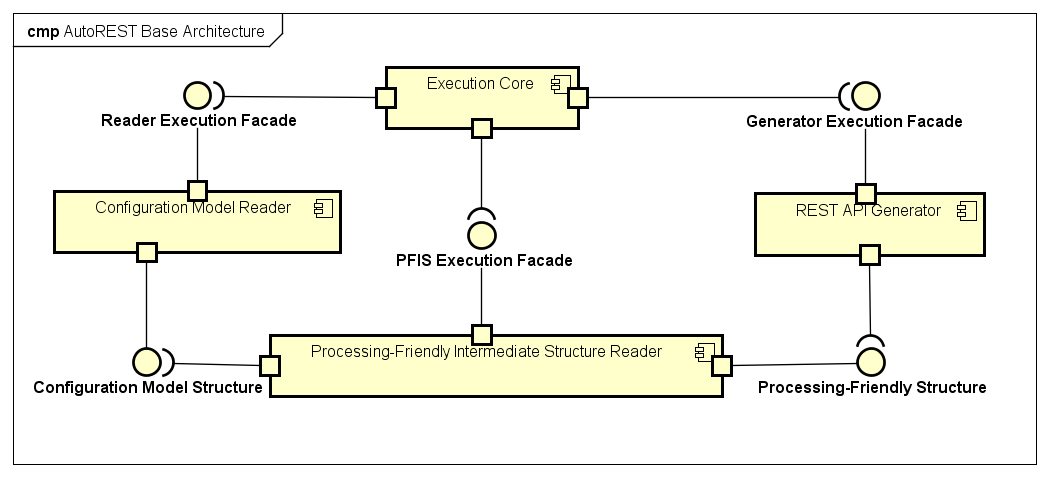
\includegraphics[scale=0.57]{imagens/AutoREST_Base_Architecture.png}
    \end{center}
	\caption{\label{fig_aba}AutoREST - Arquitetura Base}
\end{figure}

A Figura \ref{fig_aba} apresenta um diagrama de componentes UML representando os quatro subsistemas e suas interfaces. As seções a seguir descrevem cada um destes subsistemas e interfaces em maior detalhe.

\begin{itemize}
    \item \textit{Execution Core}: é o subsistema encarregado de controlar a execução da ferramenta, provendo as interfaces de usuário e gerenciando a comunicação dos outros subsistemas;
    \item \textit{Configuration Model Reader} (CMR): é o subsistema encarregado da leitura do modelo conceitual em linguagem gráfica, criado conforme orientações dadas pela documentação do componente utilizado na implementação da arquitetura;
    \item \textit{Processing-Friendly Intermediate Structure Reader} (PFIS-R): é o subsistema encarregado de realizar a tradução do modelo conceitual em linguagem gráfica para uma estrutura intermediária de fácil processamento;
    \item \textit{REST API Generator}: é o subsistema encarregado da geração de uma implementação da API REST representada no esquema conceitual de entrada do sistema;
    \item \textit{Execution Facades}: são as interfaces utilizadas para a comunicação do subsistema de controle com os outros subsistemas, definidas utilizando o padrão de projeto Fachada \cite{GAMMA:1995};
    \item \textit{Configuration Model Structure}: é a interface de comunicação entre os subsistemas CMR e PFIS-R, servindo como ponto de transferência do modelo conceitual em linguagem gráfica entre os dois subsistemas;
    \item \textit{Processing-Friendly Structure}: é a interface de comunicação entre os subsistemas PFIS-R e \textit{REST API Generator}, servindo como ponto de transferência da estrutura intermediária de fácil processamento entre os dois subsistemas.
\end{itemize}

%------------------------------------------------------------

\subsection{\textit{Execution Core} e \textit{Execution Facades}}

O subsistema \textit{Execution Core} é responsável pelo controle da aplicação através de requisições às \textit{Execution Facades}. Estas requisições devem ser procedimentos ativadores das funções básicas de cada um dos subsistemas, transferindo pacotes de dados entre eles. Estes pacotes de dados serão estruturados conforme as interfaces de estruturas providas pelos subsistemas CMR e PFIS-R.

\begin{figure}[htb]
    \begin{center}
        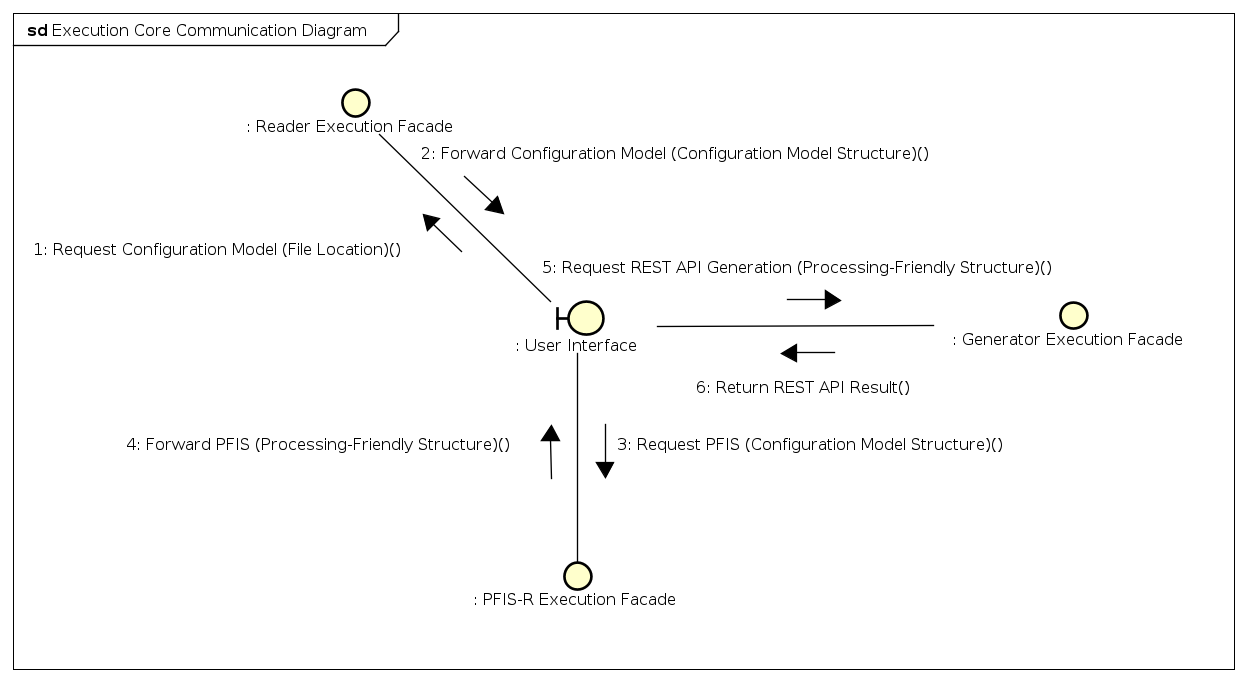
\includegraphics[scale=0.57]{imagens/Execution_Core_Communication_Diagram.png}
    \end{center}
	\caption{\label{fig_eccom}Diagrama de Comunicação do Subsistema \textit{Execution Core}}
\end{figure}

A Figura \ref{fig_eccom} apresenta um diagrama de comunicação entre a interface de usuário provida pelo \textit{Execution Core} e as interfaces de \textit{Execution Facade}. A comunicação ocorre através de cinco mensagens básicas:

\begin{enumerate}
    \item É realizada uma requisição ao \textit{Reader Execution Facade} para que o modelo conceitual, contido em um arquivo cuja localização é enviada como argumento, seja carregado em memória;
    \item Após a execução dos processos internos do subsistema CMR, o modelo conceitual é retornado ao \textit{Execution Core} para que este dê continuidade ao processo;
    \item É realizada uma requisição ao \textit{PFIS-R Execution Facade} para que o modelo conceitual em memória, contido em um pacote de dados enviado como argumento, seja convertido em uma PFIS;
    \item Após a execução dos processos internos do subsistema PFIS-R, a PFIS é retornada ao \textit{Execution Core} para que este dê continuidade ao processo;
    \item É realizada uma requisição ao \textit{Generator Execution Facade} para que a API REST seja gerada a partir do PFIS em memória, contido em um pacote de dados enviado como argumento.
\end{enumerate}

O resultado da composição do sistema através deste padrão de comportamento é um desacoplamento dos outros subsistemas componentes da arquitetura AutoREST, permitindo que estes sejam construídos de forma semi-autônoma, tendo como dependência apenas as estruturas de dados providas por interfaces de outros subsistemas.

%------------------------------------------------------------

\subsection{\textit{Configuration Model Reader} (CMR) e \textit{Configuration Model Structure}}

O subsistema \textit{Configuration Model Reader} (CMR) é responsável por definir a estrutura interna de sistema do modelo conceitual em linguagem gráfica estabelecido como modelo de configuração para uma ferramenta AutoREST, além de prover a leitura de arquivos e carga em memória destes modelos. A definição das orientações necessárias para a construção do modelo conceitual representativo da API REST que se busca gerar é dependente da implementação deste subsistema. Desta forma, é importante que a documentação de uma implementação do subsistema CMR contenha todas as orientações necessárias, conforme RQ01 apresentada na Seção \ref{sec:reqs}.

Minimamente, a estrutura de dados definida pelo subsistema CMR deve conter representações de entidades, associações entre estas identidades, seus atributos e suas restrições de integridade. Exemplos de linguagens de modelagem que proveem estes elementos são Diagramas de Classes UML anotados (utilizado na prova de conceito apresentada na Seção \ref{sec:conceptproof}) e Modelos Entidade-Relacionamento \cite{POLAK:2015} \cite{VALVERDE:2009}.

%------------------------------------------------------------

\subsection{\textit{Processing-Friendly Intermediate Structure Reader} (PFIS-R) e \textit{Processing-Friendly Structure}}

O subsistema \textit{Processing-Friendly Intermediate Structure Reader} (PFIS-R) é responsável pela tradução do modelo conceitual gráfico em um modelo textual equivalente para fácil processamento no estágio de geração da API REST, no subsistema \textit{REST API Generator}. Este subsistema é composto por três componentes, como representado na Figura \ref{fig_pfisrcom}.

\begin{figure}[htb]
    \begin{center}
        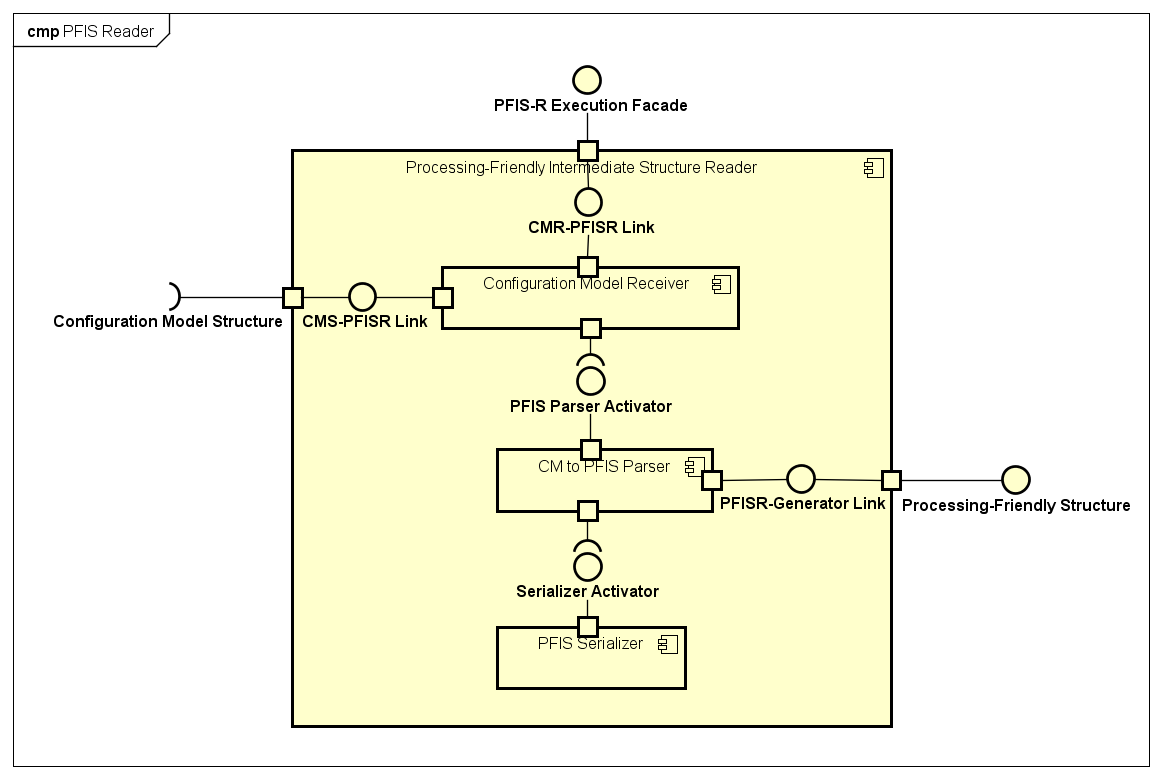
\includegraphics[scale=0.52]{imagens/PFIS_Reader_Subcomponent_Diagram.png}
    \end{center}
	\caption{\label{fig_pfisrcom}Diagrama de Componentes do Subsistema PFIS-R}
\end{figure}

As interfaces internas do subsistema, que realizam a comunicação entre os componentes, permitem um grau de autonomia entre os componentes do subsistema PFIS-R. A execução deste subsistema é descrita pelo Diagrama de Sequência apresentado nas Figuras \ref{fig_pfisrseq1} e \ref{fig_pfisrseq2}. A interface CMS-PFISR Link é omitida para reduzir o tamanho da figura.

\begin{figure}[htb]
    \begin{center}
        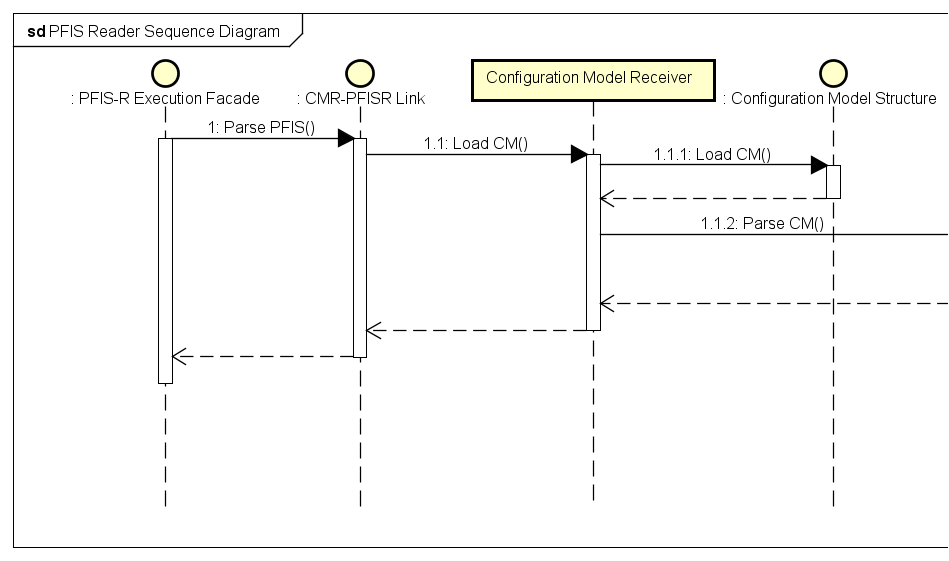
\includegraphics[scale=0.57]{imagens/PFIS_Reader_Sequence_Diagram_1.png}
    \end{center}
	\caption{\label{fig_pfisrseq1}Diagrama de Sequência do Subsistema PFIS-R - Parte 1}
\end{figure}

\begin{figure}[htb]
    \begin{center}
        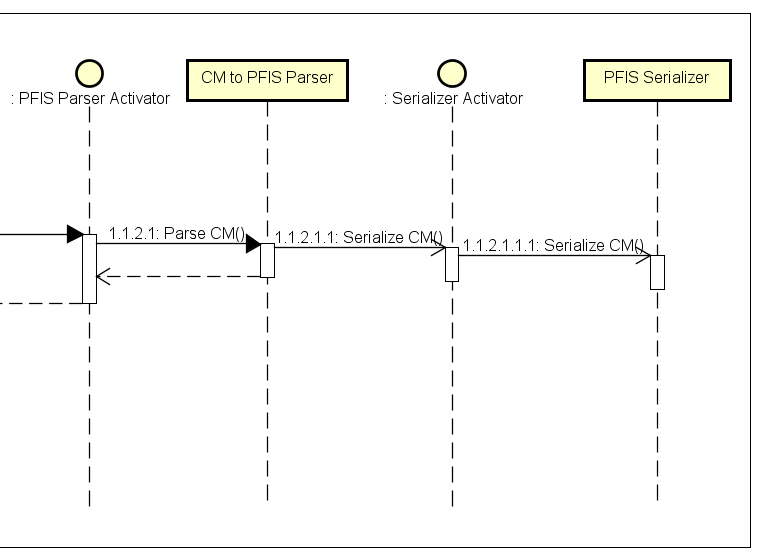
\includegraphics[scale=0.59]{imagens/PFIS_Reader_Sequence_Diagram_2.png}
    \end{center}
	\caption{\label{fig_pfisrseq2}Diagrama de Sequência do Subsistema PFIS-R - Parte 2}
\end{figure}

Este subsistema também é responsável por definir a estrutura interna de sistema da representação textual equivalente do modelo de configuração. Esta representação deve ser feita através de uma linguagem textual bem definida por terceiros, em conformidade com as definições de CBSE de \citeonline{JIFENG:2005}. Exemplos de linguagens que podem ser utilizadas para esta representação são RAML \cite{RAML}, Swagger \cite{SWAGGER}, WSDL \cite{BOOTH:2005} e JSON Schema \cite{PEZOA:2016}, este último sendo utilizado na prova de conceito apresentada na Seção \ref{sec:conceptproof}.

%------------------------------------------------------------

\subsection{\textit{REST API Generator}}

O subsistema \textit{REST API Generator} é responsável pela fase final da operação de um sistema AutoREST: a geração do código fonte de uma API REST. Este subsistema é composto por dois componentes, como apresentado na Figura \ref{fig_gencomp}: \textit{PFIS Compiler} e \textit{HTTP Method Stub Library}. O \textit{PFIS Compiler} é responsável pela execução deste subsistema, recebendo requisições através da interface \textit{Generator Execution Facade} e realizando a leitura de uma PFIS através da interface provida pelo subsistema PFIS-R.

\begin{figure}[htb]
    \begin{center}
        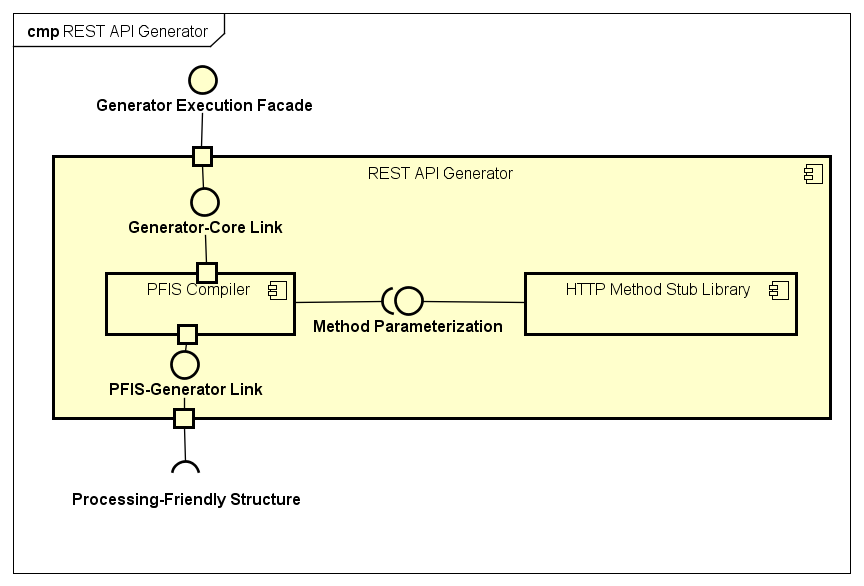
\includegraphics[scale=0.65]{imagens/REST_API_Generator_Subcomponent_Diagram.png}
    \end{center}
	\caption{\label{fig_gencomp}Diagrama de Componentes do Subsistema \textit{REST API Generator}}
\end{figure}

A partir da leitura de uma PFIS, o subsistema realiza a geração de uma API REST baseada no código parametrizável implementado na \textit{HTTP Method Stub Library}, que serve como base para todas as APIs REST geradas por uma implementação deste subsistema, oferecendo código fonte base em determinada linguagem de programação. A forma utilizada para a leitura dos artefatos de entrada pelo gerador pode variar entre implementações, o que motivou a estruturação deste subsistema de forma a permitir o reuso de uma mesma \textit{HTTP Method Stub Library} em diversas implementações deste subsistema.

%------------------------------------------------------------

\section{Prova de Conceito - Instanciando a Arquitetura AutoREST}
\label{sec:conceptproof}

Como prova de conceito da arquitetura AutoREST, será desenvolvido um sistema de geração de APIs REST baseado na arquitetura proposta, conforme as decisões de projeto delineadas na Seção \ref{sec:dds}. Este sistema irá utilizar as tecnologias de Diagramas de Classes UML, JSON Schema, Java, Node.js e MongoDB.

Os componentes de sistema serão implementados na linguagem de programação Java, utilizando o padrão \textit{Factory} \cite{GAMMA:1995} para a realização das interfaces entre subsistemas \cite{LASER:2015}. Desta forma, garante-se o desacoplamento entre os subsistemas e cria-se um ponto único no código sobre a qual gerencias comutações entre componentes, garantindo o cumprimento da RQ05.

A notação utilizada para modelos de configuração será a de Diagramas de Classes UML anotados conforme Subseção \ref{sec:xmi}, utilizando um subconjunto da linguagem JSON Schema. O artefato de entrada do subsistema instância de \textit{Configuration Model Reader} será um XML gerado pela ferramenta Astah. A utilização de UML como linguagem gráfica para o modelo de configuração garante o cumprimento da RQ01 \cite{OMG:2011}.

A notação utilizada para modelos de fácil processamento será um conjunto de definições JSON Schema, conforme Subseção \ref{sec:bnf} \cite{PEZOA:2016}. Este modelo será gerado automaticamente pelo sistema a partir do modelo de configuração, garantindo o cumprimento da RQ02.

A API REST gerada será implementada utilizando a linguagem Node.js. Um compilador será criado utilizando a ferramenta BYACC/J \cite{BYACCJ}, utilizando chamadas de função a uma biblioteca que irá conter blocos de código parametrizáveis representando os métodos HTTP. Além disso, a API REST fará uso da biblioteca Mongoose para permitir a persistência de objetos a partir do SGBD MongoDB. Desta forma, são garantidos o cumprimento das RQ03 e RQ04.

%------------------------------------------------------------

\subsection{Modelo de Configuração - Orientações de Modelagem}
\label{sec:xmi}

Para que seja possível a conversão automática de um modelo de configuração, é necessário que este tenha uma notação formal estabelecida de acordo com regras específicas. Nesta seção serão apresentadas as orientações para a modelagem de um Diagrama de Classes UML anotado, utilizando a ferramenta Astah, para que este sirva como modelo de configuração para a ferramenta AutoREST proposta. O uso de JSON Schema é majoritariamente baseado em \citeonline{DROETTBOOM:2015}. Todas as Regras de Modelagem serão indexadas como "RM\#\#" e as Regras de Conversão serão indexadas como "RC\#\#".

%------------------------------------------------------------

\subsubsection{Classe e Atributos}

Um modelo simples que pode ser utilizado como exemplo é uma única classe, sem associações, contendo apenas atributos não anotados. A Figura \ref{fig_example_class} apresenta uma classe contendo atributos de todos os tipos que serão suportados pela ferramenta.

\begin{figure}[htb]
    \begin{center}
        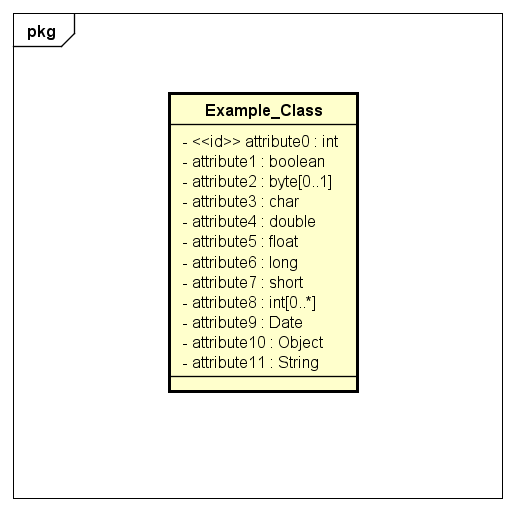
\includegraphics[scale=0.7]{imagens/Example_Class.png}
    \end{center}
	\caption{\label{fig_example_class}Classe UML - Astah}
\end{figure}

Esta classe contém doze atributos numerados de 0 a 11, sendo o primeiro (\textit{attribute0}) o identificador da classe. As seguintes regras de modelagem são estabelecidas a partir desta figura:

\begin{itemize}
    \item RM01: Todo elemento Classe deve ter um nome único dentro do escopo do diagrama, maior do que um caractere, sem espaços (utilizar CamelCase ou \_underscore).

    \item RM02: Todo elemento Classe deve ter um e apenas um atributo identificado com o Esteriótipo <<id>>, representando o atributo identificador da classe. Caso nenhum atributo seja identificado com este esteriótipo, um atributo identificador será gerado pela ferramenta AutoREST durante a conversão para JSON Schema.

    \item RM03: Todo elemento Atributo deve ter um nome único dentro do escopo da classe, maior do que um caractere, sem espaços (utilizar CamelCase ou \_underscore).

    \item RM04: A visibilidade de um elemento Atributo será ignorado pela ferramenta AutoREST, e portanto pode ser demarcado com quaisquer opções disponíveis.

    \item RM05: Um elemento Atributo pode assumir os seguintes tipos: \textit{int}; \textit{boolean}; \textit{byte}; \textit{char}; \textit{double}; \textit{float}; \textit{long}; \textit{short}; \textit{Date}; \textit{Object}; \textit{String}. Também pode ser assumido como tipo quaisquer outras Classes disponíveis no diagrama. Os tipos \textit{double} e \textit{float} serão considerados como o mesmo tipo. Os tipos \textit{int}, \textit{long} e \textit{short} serão considerados como o mesmo tipo.

    \item RM06: Um elemento Atributo com multiplicidade 0..1 será considerado como opcional.

    \item RM07: Um elemento Atributo com multiplicidade diferente de 0..1 ou 1 será considerado um vetor do tipo especificado, tal que o primeiro valor representa o tamanho mínimo do vetor (utilizar 0 para valor mínimo não definido) e o segundo valor representa o valor máximo do vetor (utilizar * para valor máximo não definido).
\end{itemize}

A partir destas regras de modelagem, podem ser estabelecidas as seguintes regras de conversão para notação JSON Schema, utilizada como PFIS:

\begin{itemize}
    \item RC01: Cada elemento Classe será convertido em um elemento de tipo \textit{object} no campo \textit{definition} de um JSON Schema, com o mesmo nome da Classe em questão.

    \item RC02: Cada elemento Atributo será convertido em um elemento de \textit{properties} de JSON Schema, com o mesmo nome do Atributo em questão.

    \item RC03: Atributos de tipo \textit{int}, \textit{short}, \textit{long} e \textit{byte} serão representados pelo tipo JSON Schema \textit{integer}. Adicionalmente, Atributos de tipo \textit{byte} serão marcados com as restrições de integridade de valor mínimo 0 e valor máximo 255.

    \item RC04: Atributos de tipo \textit{boolean} serão representados pelo tipo JSON Schema \textit{boolean}.

    \item RC05: Atributos de tipo \textit{char}, \textit{String} e \textit{Date} serão representados pelo tipo JSON Schema \textit{string}. Adicionalmente, atributos de tipo \textit{char} serão marcados com a restrição de integridade de tamanho máximo 1, e atributos de tipo \textit{Date} serão marcados com a restrição de integridade \textit{"format"\ : "date-time"}.

    \item RC06: Atributos de tipo \textit{Object} ou atributos tipados com outras Classes disponíveis no diagrama serão representados pelo tipo JSON Schema \textit{object}. Adicionalmente, atributos tipados com outras Classes disponíveis no diagrama terão como propriedade a referência da definição da respectiva Classe.

    \item RC07: Todos os atributos serão definidos como dependentes do atributo identificador.

    \item RC08: Atributos com multiplicidade diferente de 0..1 serão definidos como requeridos.

    \item RC09: Atributos com multiplicidade diferente de 0..1 ou 1 serão definidos como vetores.
\end{itemize}

%------------------------------------------------------------

\subsubsection{Restrições de integridade de atributos}

Restrições de integridade de atributos devem ser anotados diretamente nos atributos com a utilização de \textit{tags}, no formato JSON Schema. Todas as restrições de integridade aqui definidas seguem a semântica definida por \cite{PEZOA:2016}. As restrições de integridade válidas são ditadas pelas regras de construção a seguir:

\begin{itemize}
    \item RM08: Atributos de tipos \textit{int}, \textit{short} e \textit{long} podem ser anotados com as \textit{tags}: \textit{min}, \textit{max}, \textit{exMin} e \textit{exMax}.

    \item RM09: Atributos de tipo \textit{byte} e \textit{Date} não podem ser anotados, tendo em vista que estes tipos já consideram restrições de integridade próprias.

    \item RM10: Atributos de tipo \textit{boolean} não podem ser anotados, dada a natureza primitiva deste tipo.

    \item RM11: Atributos de tipo \textit{char} e \textit{String} podem ser anotados com a \textit{tag}: \textit{pattern}. Adicionalmente, atributos de tipo \textit{String} também podem ser anotados com as \textit{tags}: \textit{minLength} e \textit{maxLength}.

    \item RM12: Atributos de tipo \textit{Object} não podem ser anotados, e servem como \textit{wildcard}. Para definições de objetos mais complexos, utilizar elementos do tipo Classe.

    \item RM13: Atributos tipados com outras Classes disponíveis no diagrama não podem ser anotadas, visto que estes atributos farão referência às restrições de integridade da Classe referenciada.

    \item RM14: Atributos com multiplicidade diferente de 0..1 ou 1 (tipo vetor) podem ser anotados com a \textit{tag}: \textit{uniqueItems}, de valor booleano (\textit{true} ou \textit{false}), representando a restrição de que todos os itens do vetor sejam diferentes entre si.
\end{itemize}

Estas \textit{tags} serão convertidas diretamente para as restrições de integridade equivalentes em JSON Schema, gerando uma única regra de conversão:

\begin{itemize}
    \item RC10: Todas as \textit{tags} de elementos do tipo Atributo serão convertidas em suas respectivas restrições de integridade JSON Schema.
\end{itemize}

A Figura \ref{fig_example_tags} apresenta a parte da tela do Astah referente às \textit{tags}, com anotações referentes ao \textit{attribute11} da classe representada na Figura \ref{fig_example_class}.

\begin{figure}[htb]
    \begin{center}
        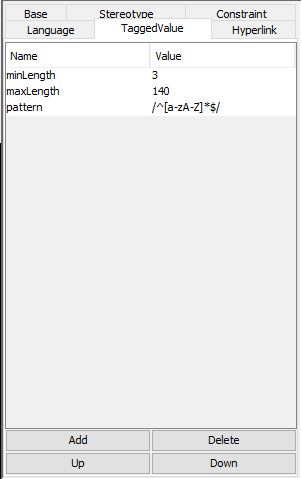
\includegraphics[scale=0.7]{imagens/Example_Tags.png}
    \end{center}
	\caption{\label{fig_example_tags}\textit{Tags} relativas ao \textit{attribute11} da Figura \ref{fig_example_class} - Astah}
\end{figure}

A partir das regras de conversão apresentadas até este ponto, a Classe representada na Figura \ref{fig_example_class} terá o formato em JSON Schema apresentado no Anexo \ref{fig_example_class_j}.

%------------------------------------------------------------

\subsubsection{Multiplicidade de Associações e Navegabilidade}

Associações simples entre duas classes podem ser representadas utilizando as notações de multiplicidade e navegabilidade. As restrições descritas nesta seção são detalhadas conforme \citeonline{BOOCH:2005}.

\begin{itemize}
    \item RM15: Associações podem ser navegáveis ou não-navegáveis. Associações anotadas como tendo navegabilidade não-definida serão considerados não-navegáveis, a menos que ambos os vértices da associação sejam de navegabilidade não-definida. Neste caso, ambos são considerados navegáveis.

    \item RM16: Associações podem ter multiplicidade 1, 0..1, 0..*, 1..* ou *. Associações de multiplicidade não definida serão consideradas como tendo multiplicidade 1.

    \item RM17: Vértices não-navegáveis de associações são considerados como tendo multiplicidade 1, independentemente da multiplicidade anotada no diagrama.
\end{itemize}

A partir destas regras de modelagem, podem ser estabelecidas as seguintes regras de conversão para notação JSON Schema, utilizada como PFIS:

\begin{itemize}
    \item RC11: Classes localizadas em vértices não-navegáveis não terão referência à classe associada.

    \item RC12: Classes localizadas em vértices navegáveis terão referência à classe associada conforme multiplicidade do vértice.

    \item RC13: Vértices de multiplicidade 1 ou 0..1 serão representados pela adição do(s) atributo(s) identificador(es) da classe associada à sua especificação. Adicionalmente, vértices de multiplicidade 0..1 terão este atributo identificador representado como opcional.

    \item RC14: Vértices de multiplicidade 0..*, * ou 1..* serão representados pela adição de vetores do(s) atributo(s) identificador(es) da classe associada à sua especificação. Adicionalmente, vértices de multiplicidade 1..* terão adicionada a este vetor a restrição de integridade de tamanho mínimo 1.
\end{itemize}

\begin{figure}
    \begin{center}
        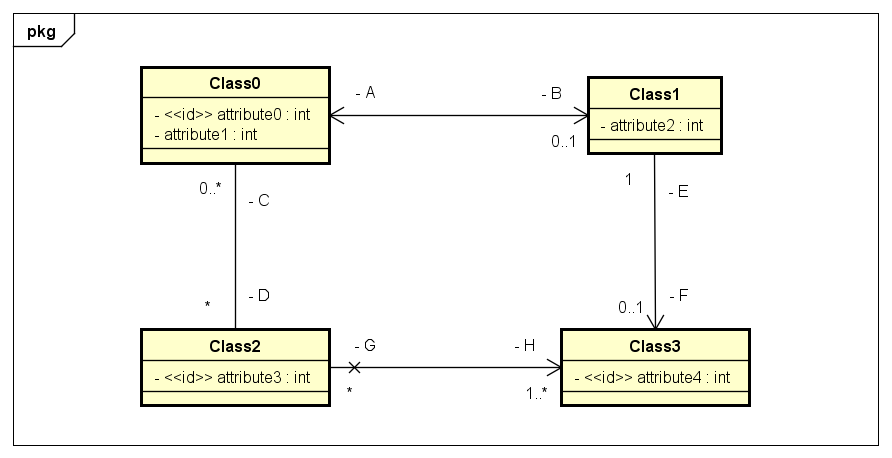
\includegraphics[scale=0.7]{imagens/Example_Multiplicity.png}
    \end{center}
	\caption{\label{fig_example_multiplicity}Exemplo de Diagrama de Classes UML com Associações Simples - Astah}
\end{figure}

A Figura \ref{fig_example_multiplicity} apresenta um exemplo de diversas possíveis aplicações de associações simples à um diagrama. O resultado da conversão deste diagrama é apresentado no Anexo \ref{fig_example_multiplicity_j}. A seguir é apresentada a aplicação das regras de conversão descritas até este ponto:

\begin{itemize}
    \item Cada uma das classes tem um elemento criado em \textit{definitions}, conforme RCs 1-10.

    \item \textit{Class1} tem um atributo identificador criado, visto que não possui nenhum atributo anotado com o esteriótipo <<id>>, conforme RM 2.

    \item \textit{Class0} tem adicionado as suas propriedades o atributo identificador de \textit{Class1} anotado como opcional, dado o vértice navegável B de multiplicidade 0..1, conforme RC13.

    \item \textit{Class0} tem adicionado as suas propriedades um vetor do atributo identificador de \textit{Class2} anotado como opcional, dado o vértice de navegabilidade não definida D de multiplicidade *, conforme RM 15 e RC14.

    \item \textit{Class1} tem adicionado as suas propriedades o atributo identificador de \textit{Class0} anotado como opcional, dado o vértice navegável A de multiplicidade não definida, conforme RM 16 e RC 13.

    \item \textit{Class1} tem adicionado as suas propriedades o atributo identificador de \textit{Class3} anotado como opcional, dado o vértice navegável F de multiplicidade 0..1, conforme RC 13.

    \item \textit{Class2} tem adicionado as suas propriedades um vetor do atributo identificador de \textit{Class0} anotado como opcional, dado o vértice de navegabilidade não definida C de multiplicidade 0..*, conforme RM 15 e RC 14.

    \item \textit{Class2} tem adicionado as suas propriedades um vetor do atributo identificador de \textit{Class3} com tamanho mínimo 1, dado o vértice navegável H de multiplicidade 1..*, conforme RC 14.

    \item \textit{Class3} não tem adicionado as suas propriedades um vetor do atributo identificador de \textit{Class2}, dado o vértice não navegável G de multiplicidade *, conforme RMs 15 e 17.

    \item \textit{Class3} não tem adicionado as suas propriedades o atributo identificador de \textit{Class1}, dado o vértice de navegabilidade não definida E de multiplicidade 1, conforme RM 15.
\end{itemize}

%------------------------------------------------------------

\subsubsection{Associações de Generalização/Especialização}

Associações de Generalização/Especialização permitem o reuso e a extensão de classes representadas no modelo de configuração. As restrições aplicadas a este tipo de associação são:

\begin{itemize}
    \item RM18: Uma classe pode ser uma Especialização de uma e apenas uma outra classe, não sendo permitida a modelagem de herança múltipla para fins desta ferramenta.

    \item RM19: Todas as associações de Generalização/Especialização são consideradas Parciais e Não-exclusivas.

    \item RM20: Uma classe "filha"\ não pode ter atributos identificadores, sendo estes necessariamente herdados da classe "pai".
\end{itemize}

É necessária uma única regra de conversão para que este tipo de associação seja contemplado:

\begin{itemize}
    \item RC15: A classe "filha"\ de uma associação de Realização/Especialização será representada em JSON Schema pela composição de seus atributos e uma referência à classe "pai".
\end{itemize}

A razão da ferramenta AutoREST utilizar apenas um subconjunto restrito das associações de Generalização/Especialização é descrita no Capítulo \ref{chap:concl}. A Figura \ref{fig_example_realization} apresenta um exemplo válido de diagrama de classes utilizando associações de Especialização/Generalização. O JSON Schema relacionado é apresentado no Anexo \ref{fig_example_realization_j}.

\begin{figure}
    \begin{center}
        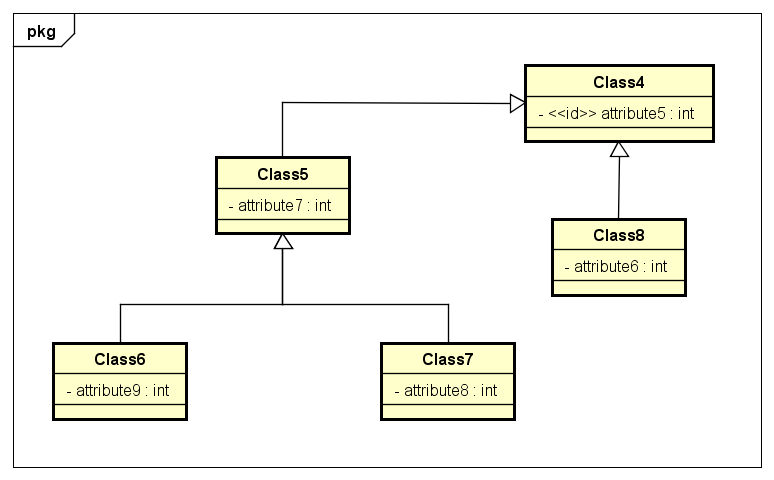
\includegraphics[scale=0.7]{imagens/Example_Realization.png}
    \end{center}
	\caption{\label{fig_example_realization}Exemplo de Diagrama de Classes UML com Associações de Generalização/Especialização - Astah}
\end{figure}

%------------------------------------------------------------

\subsubsection{Associações de Agregação}

Associações de Agregação permitem a representação de posse de uma classe sobre outra. Dois tipos de agregação são permitidos: Agregação Simples e Agregação por Composição. As restrições aplicadas a este tipo de associação são:

\begin{itemize}
    \item RM21: Associações de Agregação Simples representam a posse de uma classe sobre outra, porém mantendo a independência funcional de cada uma das classes associadas.

    \item RM22: Associações de Agregação por Composição representam a posse de uma classe sobre outra, sendo a classe "possuída"\ uma definição interna da classe "possessora". Desta forma, a classe possuída só pode existir no contexto da classe possessora.

    \item RM23: O vértice possuído de Associações de Agregação pode ter multiplicidade 1, 0..1, 0..*, * ou 1..*.

    \item RM24: O vértice possessor de Associações de Agregação deve ter multiplicidade 1.

    \item RM26: Não é comportada navegabilidade direcionada da classe possuída para a classe possessora, por limitação da notação gráfica da ferramenta Astah. Por esta razão, assume-se sempre navegabilidade bidirecional para Agregação Simples e unidirecional para Agregação por Composição.
\end{itemize}

São estabelecidas as seguintes regras de conversão para que este tipo de associação seja contemplado:

\begin{itemize}
    \item RC16: O vértice possuído de Associações de Agregação, quando navegável, será representado da mesma forma descrita pelas RCs 11-14.

    \item RC17: O vértice possessor de Associações de Agregação Simples será representado por uma referência à classe possuída, ou um vetor de referências à classe possuída, definido de acordo com a multiplicidade do vetor, de forma similar a RCs 13-14.

    \item RC18: O vértice possessor de Associações de Agregação por Composição será representado por uma definição interna de classe, seguindo as regras de multiplicidade das RCs 13-14 para decisão de uso de definição única ou vetor.

    \item RC19: Classes possuídas de Associações de Agregação por Composição não serão representadas nas definições base.
\end{itemize}

A Figura \ref{fig_example_aggregation} apresenta um diagrama de classes que utiliza os dois tipos de associação de agregação, além de um tipo de associação simples para que seja possível visualizar a diferença entre estes. O Anexo \ref{fig_example_aggregation_j} apresenta o JSON Schema resultante da conversão deste diagrama.

\begin{figure}
    \begin{center}
        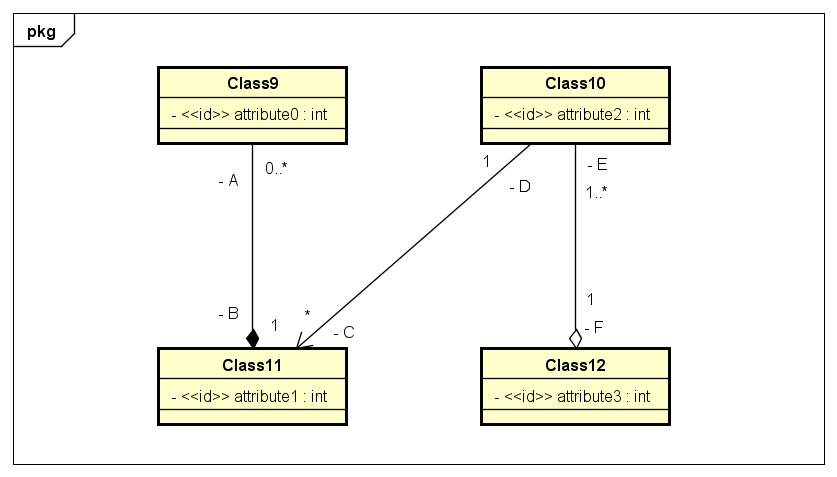
\includegraphics[scale=0.7]{imagens/Example_Aggregation.png}
    \end{center}
	\caption{\label{fig_example_aggregation}Exemplo de Diagrama de Classes UML com Associações de Agregação - Astah}
\end{figure}

%------------------------------------------------------------

\subsubsection{Classes Associativas}

Classes Associativas podem ser utilizadas para representar associações entre classes que contém atributos próprios. A seguinte restrição se aplica:

\begin{itemize}
    \item RM27: Classes Associativas não podem possuir atributo identificador; os identificadores das classes associadas são utilizados.
\end{itemize}

As regras de conversão referentes a esta restrição são:

\begin{itemize}
    \item RC20: Cada uma das classes associadas irá receber um vetor de referências à objetos da classe associativa.

    \item RC21: Um objeto será criado em \textit{definitions} para a classe associativa, utilizando como identificador a composição dos identificadores das classes associadas.
\end{itemize}

A Figura \ref{fig_example_association_class} apresenta um diagrama de classes exemplo. O Anexo \ref{fig_example_association_class_j} apresenta o JSON Schema resultante da conversão deste diagrama.

\begin{figure}
    \begin{center}
        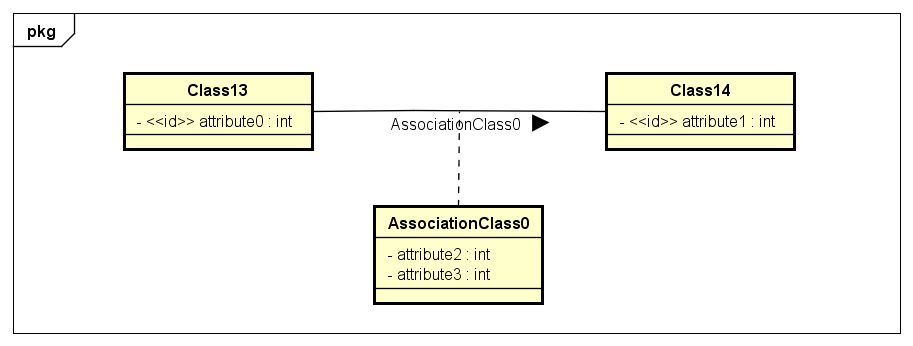
\includegraphics[scale=0.7]{imagens/Example_Association_Class.png}
    \end{center}
	\caption{\label{fig_example_association_class}Exemplo de Diagrama de Classes UML com Classe Associativa - Astah}
\end{figure}

%------------------------------------------------------------

%\subsection{Algoritmo de Geração de JSON Schema a partir de XML}

%A ferramenta AutoREST implementada como prova de conceito deste estudo irá utilizar um subconjunto dos elementos de Diagramas de Classes UML descritos em \cite{OMG:2011}, modelado na ferramenta Astah, para a criação de um arquivo JSON Schema de acordo com \citeonline{PEZOA:2016}. Este subconjunto e sua interpretação semântica na ferramenta AutoREST estão descritos a seguir, assim como as regras de modelagem que devem ser seguidas para que o diagrama seja válido como artefato de entrado do sistema AutoREST.

%\begin{itemize}
%    \item Classe: Representa um elemento do tipo \textit{object} em JSON Schema e uma \textit{collection} em MongoDB. Não possui restrições de nomenclatura.
%    \item Atributo de Classe: Representa uma propriedade da classe em JSON Schema. Atributos de Classe devem ser tipados corretamente como: int, representando o tipo JSON "integer"; float, representando "number"; string, ou; boolean. Para atributos que serão usados como chave primária, o nome deve ser escrito "\textless nome\textgreater \_id". Atributos usados como chave estrangeira serão sub-entendidos a partir dos relacionamentos utilizados. O caso particular de atributos do tipo "DateTime"\ devem ser tipados como float.
%    \item Associação: É entendida pelo sistema como representação de chaves estrangeiras, de acordo com a cardinalidade utilizada, da seguinte forma: para associações 0..*, a classe representada no ponto oposto da associação terá como chave estrangeira um vetor com as chaves primárias da classe representada no ponto 0..* da associação. Associações *..* terão chaves estrangeiras em ambos os pontos da associação. Associações 1..* terão como chave estrangeira a chave primária do ponto da associação 1, representado no ponto da associação *. Associações 1..1 não são suportadas. Todas as chaves estrangeiras criadas pelo sistema tem o formato "\textless nome\textgreater \_fk".
%    \item Associação de Composição: É entendida pelo sistema como representando, na classe "agregada", uma classe interna. É representada em JSON Schema utilizando o tipo de recurso "refSch".
%    \item Classe Associativa: É entendida pelo sistema como um "object"\ cuja chave primária é composta pelas chaves estrangeiras advindas das classes a que está associada. Estas chaves estrangeiras são representadas com a string "\textless nome\textgreater \_fk" e sub-entendidas pelo gerador de código como chave primária composta.
%\end{itemize}

%Além destas notações, o sistema AutoREST espera uma notação em formato de "tag"\ para algumas especificações de propriedades JSON. As tags aceitas pelo sistema são:

%\begin{itemize}
%    \item minLength: Específico para propriedades de tipo string, representa o tamanho mínimo da string. Deve ser anotado em formato numérico.
%    \item maxLength: Específico para propriedades de tipo string, representa o tamanho máximo da string. Deve ser anotado em formato numérico.
%    \item pattern: Específico para propriedades de tipo string, representa o padrão que deve ser seguido pela string. Deve ser anotado em formato de expressão regular.
%    \item minimum: Específico para propriedades de tipo integer e number, representa o valor mínimo da propriedade. Deve ser anotado em formato numérico.
%    \item maximum: Específico para propriedades de tipo integer e number, representa o valor máximo da propriedade. Deve ser anotado em formato numérico.
%    \item exclusiveMinimum: Específico para propriedades de tipo integer e number, classifica se o valor especificado como mínimo é inclusivo ou não. Deve ser representada com o valor booleano true ou false. Caso não esteja presente, assume-se como false.
%    \item exclusiveMaximum: Específico para propriedades de tipo integer e number, classifica se o valor especificado como máximo é inclusivo ou não. Deve ser representada com o valor booleano true ou false. Caso não esteja presente, assume-se como false.
%\end{itemize}

%O algoritmo utilizado para a conversão do formato XMI para o formato JSON Schema é descrito abaixo, em formato de pseudo-código.

%\begin{algorithm}
%\caption{Pseudo-código da tradução de XMI para JSON Schema}
%\begin{algorithmic}
%    \ForAll{Classes}
%        \State Create new JSON Schema object
%        \ForAll{Attributes}
%            \State Create new JSON Schema property
%            \If{Attribute has Tags}
%                \State Create appropriate restrictions
%            \EndIf
%        \EndFor
%    \EndFor
%
%    \ForAll{Associations}
%        \State Create appropriate foreign keys
%    \EndFor
%
%    \State Create definition block
%\end{algorithmic}
%\end{algorithm}

%------------------------------------------------------------

\subsection{Gramática BNF para Geração de Código a partir de JSON Schema}
\label{sec:bnf}

Em \cite{PEZOA:2016} é definida e validada formalmente uma gramática na forma de Backus-Naur (BNF), para a estrutura JSON Schema \citeonline{GALIEGUE:2013}. A seguir serão exploradas as partes desta gramática utilizadas no subsistema \textit{REST API Generator} e seu significado semântico.

%------------------------------------------------------------

\subsubsection{Sintaxe}
A gramática BNF irá ser usada como entrada para a geração de um \textit{parser} na ferramenta BYACC/J \cite{BYACCJ}. O subconjunto de definições que serão relevantes para o subsistema está contido na definição \textit{defs}, que corresponde à propriedade \textit{definitions} de um JSON Schema. Cada \textit{defs} possui no minimo um \textit{kSch}, que é composto de um nome (\textit{kword}) e uma ou mais restrições (\textit{res}). Conforme segmento extraído de \cite{PEZOA:2016}:

\begin{algorithmic}
    \item \textbf{defs} := "definitions": \{ \textbf{kSch} (, \textbf{kSch})*\}
    \item \textbf{kSch} := \textbf{kword}: \{ \textbf{JSch} \}
    \item \textbf{JSch} := ( \textbf{res} (, \textbf{res})*)
    \item \textbf{res} := \textbf{type} | \textbf{strRes} | \textbf{numRes} | \textbf{arrRes} | \textbf{objRes} | \textbf{multRes} | \textbf{refSch} | \textbf{title} | \textbf{description}
\end{algorithmic}

A gramática utilizada serve para a validação sintática completa de um JSON Schema, porém somente algumas das definições terão significado semântico para o subsistema, conforme seção a seguir. A gramática completa está no Anexo \ref{anexo:bnfjs}.

\subsubsection{Semântica}

Nesta seção serão apresentadas as derivações \textit{kSch}, que deriva de \textit{defs}, consideradas no processo de criação da API REST, assim como suas derivações utilizadas. Depois serão apresentados os processos de geração do código fonte final, subseções \ref{sec:bnf:http} e \ref{sec:bnf:mongo}.

%Todas as 'definitions' devem estar no primeiro nivel e somente serem referenciadas referenciadas nos niveis abaixo
%Verificar termos abaixo desta derivação que serão ignorados, por nao se aplicarão a nossa ferramenta, candicados possiveis sao as restrições de multiplicidade

\subsubsubsection{Derivações de \textit{kSch}}
\label{sec:bnf:ksch}

Cada \textit{kSch} será considerada a definição de um \textit{resource} a ser fornecido pela API, logo a derivação \textit{kword} se tornará o nome deste \textit{resource} e a derivação \textit{JSch} será utilizada para a geração de métodos HTTP disponibilizados para o \textit{resource} e para a criação de um \textit{model} do modulo Mongoose de Node.js, que subsequentemente irá fazer as iterações com o MongoDB. As derivações utilizadas para um \textit{JSch} de um \textit{resource} serão:
\begin{itemize}
    %\item \textbf{title}: título do \textit{resource}

    %\item \textbf{description}: descrição do \textit{resource}

    \item \textbf{type}: restringe o tipo do objeto sendo definido, para um \textit{resource} o valor deverá ser \textit{object}, outros valores serão considerados inválidos
    %\item \textbf{strRes}: restrições aplicáveis a \textit{strings}
    %\item \textbf{numRes}: restrições aplicáveis a números (inteiros e decimais)
    %\item \textbf{arrRes}: restrições a \textit{arrays}

    \item \textbf{objRes}: restrições do \textit{resource}, serão consideradas as definições na Subseção \ref{sec:bnf:obj}
    %\item \textbf{multRes}: restrições de multiplicidade, enumerações, conjunções e disjunções
    %\item \textbf{refSch}: referências a outros \textit{schemas}, seja localmente ou em outro arquivo
\end{itemize}

\subsubsubsection{Derivações de \textit{objRes}}
\label{sec:bnf:obj}
A diretiva \textit{objRes} representa as restrições relacionadas a definição de um objeto, ela pode ser usada tanto para definição de \textit{resources} quanto para a definição de propriedades do tipo objeto. As derivações consideradas válidas são as seguintes:

\begin{itemize}
    \item \textbf{properties}: irá conter as propriedades do objeto sendo definido, será melhor detalhada na Seção \ref{sec:bnf:props}.

    %\item \textbf{additionalProperties}: indica se o objeto poderá conter propriedades adicionais, para esta derivação é esperado somente um valor booleano (\textit{true} ou \textit{false}), outros valores serão considerados inválidos

    \item \textbf{required}: define quais propriedades são obrigatórias

    \item \textbf{dependencies}: será considerada nesta diretiva somente a derivação contendo um \textit{kArr}, que é o nome de uma propriedade e suas dependências, todas as propriedades serão dependentes da propriedade definida como chave primária, para que a chave primária seja composta será necessario que as propriedades sejam dependentes de mais de uma propriedade
\end{itemize}

\subsubsubsection{Derivações de \textit{properties}}
\label{sec:bnf:props}
As propriedades de um objeto serão todas as derivações \textit{kSch} que fazem parte da diretiva \textit{properties} relacionada ao mesmo. Porém as derivações de um \textit{kSch} terão um significado diferente quando aplicadas a uma propriedade, do que quanto aplicadas a um \textit{resource}. A derivação \textit{kword} será o nome da propriedade e para a derivação \textit{JSch} serão consideradas válidas somente as derivações listadas a seguir:
\begin{itemize}
    %\item \textbf{title}: título da propriedade

    %\item \textbf{description}: descrição da propriedade

    \item \textbf{type}: restringe o tipo da propriedade sendo definida, caso nenhum valor seja informado assume-se \textit{object}. Valores considerados válidos são: \textit{string}, \textit{integer}, \textit{number}, \textit{boolean}, \textit{object} e \textit{array}.

    \item \textbf{strRes}: será aceita quando o \textit{type} for \textit{string} e serão consideradas válidas as seguintes derivações:
    \begin{itemize}
        \item \textbf{minLength}: tamanho minimo do valor da propriedade
        \item \textbf{maxLength}: tamanho máximo do valor da propriedade
        %\item \textbf{pattern}: expressão regular para validação do valor
    \end{itemize}

    \item \textbf{numRes}: será aceita quando o \textit{type} for \textit{integer} ou \textit{number} e serão consideradas válidas as seguintes derivações:
    \begin{itemize}
        \item \textbf{minimum}: valor minimo da propriedade
        \item \textbf{exclusiveMinimum}: valor booleano, indica se o valor minimo está incluído ou não no intervalo de validação
        \item \textbf{maximum}: valor máximo da propriedade
        \item \textbf{exclusiveMaximum}: valor booleano, indica se o valor máximo está incluído ou não no intervalo de validação
    \end{itemize}

    \item \textbf{arrRes}: será aceita quando o \textit{type} for \textit{array}, será melhor detalhada na Subseção \ref{sec:bnf:arr}

    \item \textbf{objRes}: será aceita quando o \textit{type} for \textit{object} e então serão aplicadas as definições da Subseção \ref{sec:bnf:obj}
    %\item \textbf{multRes}: restrições de multiplicidade, enumerações, conjunções e disjunções

    \item \textbf{refSch}: referências a outros definições no arquivo JSON Schema que esta sendo processado, estas referencias possuirão significados diferentes, de acordo com seu contexto, na disponibilização dos \textit{resources} pela API, conforme Seções \ref{sec:bnf:mongo} e \ref{sec:bnf:http}
\end{itemize}

\subsubsubsection{Derivações de \textit{arrRes}}
\label{sec:bnf:arr}
As restrições desta diretiva são relacionadas ao \textit{type array} e serão aceitas as seguintes derivações:
\begin{itemize}
    \item \textbf{items}: definição dos tipos do \textit{array} e pode ser derivada de duas formas:
    \begin{itemize}
        \item \textbf{sameitems}: determina que todos os itens do \textit{array} possuem a mesma definição, que é determinada por um \textit{JSch}, e para esta definição são aceitas as mesmas derivações de \textit{JSch} da Subseção \ref{sec:bnf:props}

        \item \textbf{varitems}: determina que o \textit{array} pode ter itens de definições variadas, esta derivação será considerada inválida pelo gerador

    \end{itemize}

    %\item \textbf{additems}: é uma derivação que espera um valor booleano e opcional pois

    \item \textbf{minitems}: indica o numero minimo de itens do \textit{array}

    \item \textbf{maxitems}: indica o numero máximo de itens do \textit{array}
\end{itemize}


\subsubsubsection{Geração dos \textit{models} Mongoose}
\label{sec:bnf:mongo}

Para a criação dos \textit{models} de cada \textit{resource} serão usadas as seguintes regras de criação:
\begin{itemize}
    \item Cada propriedade do \textit{resource} no JSON Schema irá resultar em uma propriedade do \textit{model} Mongoose

    \item Uma propriedade do tipo \textit{integer} no JSON Schema resultará em uma propriedade Mongoose com propriedades \textit{type: Number} e \textit{integer: true}

    \item Uma propriedade do tipo \textit{number} no JSON Schema resultará em uma propriedade Mongoose com a propriedade \textit{type: Number}

    \item Uma propriedade do tipo \textit{boolean} no JSON Schema resultará em uma propriedade Mongoose com a propriedade \textit{type: Boolean}

    \item Uma propriedade do tipo \textit{string} no JSON Schema resultará em uma propriedade Mongoose com a propriedade \textit{type: String}

    \item Uma propriedade do tipo \textit{array} no JSON Schema resultará em uma propriedade Mongoose com uma propriedade \textit{any} que será um \textit{array} contendo o \textit{SchemaType} Mongoose dos elementos

    \item Uma propriedade do tipo \textit{object} no JSON Schema resultará em uma propriedade Mongoose com a propriedade \textit{type: Object}, se esta propriedade \textit{object} possuir definições JSON Schema, esta serão criadas no Mongoose conforme estas mesmas regras

    \item Todas as propriedades do JSON Schema especificadas como \textit{required} receberão uma propriedade Mongoose \textit{required: true}

    \item Todas as propriedades do JSON Schema dos tipos \textit{number} e \textit{integer} que possuirem definições de máximo e minimo receberão propriedades Mongoose correspondentes

    \item Propriedades do JSON Schema do tipo \textit{string} que possuírem definições de tamanho máximo e tamanho minimo receberão propriedades Mongoose correspondentes

\end{itemize}

As definições \textit{dependencies} do JSON Schema são interpretadas como se referindo a chave primária de um \textit{resource}, logo a propriedade da qual todas as outras dependem será considerada a chave primária. O MongoDB considera como chave primária de suas \textit{collections} a propriedade \textit{\_id} e este comportamento é assimilado pelo Mongoose.

Se for identificado que um \textit{resource} possui uma chave primária composta por mais de uma propriedade, ele receberá um \textit{index unique} que contenha todas estas propriedades que compõem a chave, fazendo-o assim respeitar a restrição de unicidade da chave primária.

Para \textit{arrays} e propriedades que possuam referencias (\textbf{refSch}) a outros \textit{resources} a criação do \textit{model} sofrerá alterações. Se um \textit{array} possuir itens que são referencias (\textbf{refSch}) a outro \textit{resource} então o que será armazenado no MongoDB serão os valores das chaves primárias deste \textit{resource}, e o \textit{model} Mongoose possuirá propriedades correspondentes. Quando uma propriedade for referencia a outro \textit{resource} isto implicará em uma herança, então o \textit{model} que contem esta propriedade será armazenado na mesma \textit{collection} no MongoDB e possuirá seu \textit{Schema} de Mongoose representando o relacionamento de herança.

Para que os \textit{resources} fornecidos pela API não contenham propriedades não desejadas, e ainda seja possível utilizar a chave primária com seu nome original, serão utilizados métodos de acesso virtuais do Mongoose. Como exemplo temos o atributo \textit{attribute0} da classe apresentada na Figura \ref{fig_example_class} no Listing \ref{lst_virtual}, o código completo para o \textit{model} desta classe está no Anexo \ref{anexo:model_mongoose}.

\begin{listing}
\begin{minted}[frame=single,
                framesep=3mm,
                linenos=true,
                xleftmargin=21pt,
                breaklines=true,
                tabsize=4]{js}
Example_ClassSchema.virtual('attribute0').get(function() {
    return this._id;
});
Example_ClassSchema.virtual('attribute0').set(function (value) {
    this._id = value;
});
\end{minted}
\caption{Exemplo métodos virtuais Mongoose}
\label{lst_virtual}
\end{listing}

Além da propriedade \textit{\_id} do MongoDB o Mongoose também adiciona outras propriedades que não estariam de acordo com o JSON Schema do \textit{resoruce}, para evitar o envio destas propriedades todos os \textit{models} possuirão o método \textit{cleanObject} que terá a função de retornar um objeto sem estas propriedades, um exemplo aplicado a classe \textit{Example\_Class} pode ser visto no Listing \ref{lst_clean_obj}.

\begin{listing}
\begin{minted}[frame=single,
                framesep=3mm,
                linenos=true,
                xleftmargin=21pt,
                breaklines=true,
                tabsize=4]{js}
Example_ClassSchema.methods.cleanObject = function() {
    var doc = this.toObject({ virtuals: true });
    delete doc.__v;
    delete doc._id;
    delete doc.id;
    return doc;
};
\end{minted}
\caption{Exemplo método \textit{cleanObject}}
\label{lst_clean_obj}
\end{listing}

\subsubsubsection{Geração dos métodos HTTP}
\label{sec:bnf:http}

Cada \textit{resource} terá seus métodos HTTP dentro de um \textit{middleware} do tipo \textit{Router}, que será utilizado pelo módulo \textit{Express} do \textit{Node.js} para gerenciar as \textit{requests}.

Os métodos HTTP gerados para um \textit{resource} serão todos os identificados como necessários para realizar as operações CRUD, que são: GET, HEAD, POST, PUT, PATCH e DELETE.

Um \textit{resource} com uma chave primária simples possuirá os \textit{endpoints} apresentados na Tabela \ref{tab:http_1}, onde: \textit{resourceName} é o nome do \textit{resource}, e; \textit{idendifier} é a chave primária do resource. As \textit{query strings} nas URIs indicadas são opcionais e os parâmetros esperados seriam \textit{propName}, que é o nome de uma propriedade, e \textit{valueX}, que é o valor desejado na propriedade; é possível mais de um parâmetro de filtro na \textit{query string}.

\begin{table}[]
    \centering
    \begin{tabularx}{\textwidth}{|l|l|X|}
        \hline
        \textbf{Método} & \textbf{URI} & \textbf{Função} \\
        \hline

        GET & /resourceName/[?propName=valueX]            & Retornar todos os \textit{resources} da \textit{collection}\\
        \hline

        GET & /resourceName/:idendifier & Retornar o \textit{resource} com o \textit{idendifier} igual ao parâmetro na URI\\
        \hline

        HEAD & /resourceName/:idendifier & Verificar se o \textit{resource} com o \textit{idendifier} igual ao parâmetro indicado existe, sem retorna-lo\\
        \hline

        POST & /resourceName/ & Inserir ou modificar totalmente o \textit{resource} contido no \textit{message body} da \textit{request}\\
        \hline

        PUT & /resourceName/:idendifier & Inserir ou modificar totalmente o \textit{resource} indicado pelo parâmetro da URI, utilizando os dados contidos no \textit{message body} da \textit{request}\\
        \hline

        PATCH & /resourceName/:idendifier & Modificar parcialmente o \textit{resource} indicado pelo parâmetro da URI, utilizando os dados contidos no \textit{message body} da \textit{request}\\
        \hline

        DELETE & /resourceName/:idendifier & Excluir o \textit{resource} com o \textit{idendifier} igual ao parametro indicado\\
        \hline
    \end{tabularx}
    \caption{\textit{Resource} Simples - Métodos HTTP e URIs}
    \label{tab:http_1}
\end{table}

Se um \textit{resource} possuir uma chave composta, seus \textit{endpoints} ao invés de aceitarem um \textit{identifier} irão esperar que os valores das chaves sejam enviados via \textit{query string}; e o comportamento gerado para o caso de nem todas as chaves serem enviadas na \textit{query string} será de um erro retornado ao cliente. Estas alterações nos \textit{endpoints} são apresentadas na Tabela \ref{tab:http_2}; a função dos métodos permanecem as mesmas.

\begin{table}[]
    \centering
    \begin{tabularx}{\textwidth}{|l|l|X|}
        \hline
        \textbf{Método} & \textbf{URI} & \textbf{\textit{Query string}} \\
        \hline

        GET & /resourceName/[?propName=valueX] & Opcional, utilizado somente para filtro, aplicável a todas as propriedades\\
        \hline

        HEAD & /resourceName/[?propName=valueX] & Devem ser informados os valores da chave primária\\
        \hline

        POST & /resourceName/ & Não aplicável (mantém comportamento utilizando o \textit{message body})\\
        \hline

        PUT & /resourceName/[?propName=valueX] & Devem ser informados os valores da chave primária\\
        \hline

        PATCH & /resourceName/[?propName=valueX] & Devem ser informados os valores da chave primária\\
        \hline

        DELETE & /resourceName/[?propName=valueX] & Devem ser informados os valores da chave primária\\
        \hline
    \end{tabularx}
    \caption{\textit{Resource} com chave composta - Métodos HTTP e URIs}
    \label{tab:http_2}
\end{table}

Quando um \textit{resource} com chave primária simples possuir propriedades complexas, ou do tipo \textit{array}, estas poderão ser acessadas diretamente através de \textit{endpoints} dedicados a elas se o \textit{endpoint} já possuir o \textit{identifier} do \textit{resource}. Estes \textit{endpoints} serão formados utilizando o \textit{endpoint} do \textit{resource} e um sufixo com o nome da propriedade, conforme Tabela \ref{tab:end_prop}. Propriedades complexas que estão contidas dentro de outras propriedades complexas possuirão seus \textit{endpoints} também, sendo estes criados com o mesmo procedimento, adicionando um sufixo com o nome da propriedade aos \textit{endpoints} já existentes.

\begin{table}[]
    \centering
    \begin{tabularx}{\textwidth}{|l|l|X|}
        \hline
        \textbf{Método} & \textbf{URI} & \textbf{\textit{Query string}} \\
        \hline

        GET & /resourceName/:idendifier/propName & Retornar o conteúdo da propriedade \textit{propName} do \textit{resource} com o \textit{idendifier} igual ao parâmetro na URI\\
        \hline

        HEAD & /resourceName/:idendifier/propName & Verificar se o \textit{resource} com o \textit{idendifier} igual ao parâmetro indicado existe e possui a propriedade \textit{propName}, sem retornar seu valor\\
        \hline

        PUT & /resourceName/:idendifier/propName & Inserir ou modificar totalmente o conteúdo da propriedade \textit{propName} no \textit{resource} indicado pelo parâmetro da URI, utilizando os dados contidos no \textit{message body} da \textit{request}\\
        \hline

        PATCH & /resourceName/:idendifier/propName & Modificar parcialmente o conteúdo da propriedade \textit{propName} do \textit{resource} indicado pelo parâmetro da URI, utilizando os dados contidos no \textit{message body} da \textit{request}. Não aplicável a propriedades \textit{array}\\
        \hline

        DELETE & /resourceName/:idendifier/propName & Excluir a propriedade \textit{propName} do \textit{resource} com o \textit{idendifier} igual ao parâmetro indicado\\
        \hline
        \hline
    \end{tabularx}
    \caption{\textit{Endpoints} de propriedades complexas e \textit{arrays}}
    \label{tab:end_prop}
\end{table}

%A API gerada irá possuir ... status codes


\subsection{Funcionamento da API REST gerada}

A API gerada poderá ser utilizada através de um arquivo "\textit{api.js}"\ que será gerado após todos os \textit{models} e \textit{routers} serem gerados. Neste arquivo o servidor \textit{Express} será criado e iniciado e os \textit{routers} gerados serão adicionados como \textit{middleware} do servidor. Também constarão no arquivo a criação da conexão com o MongoDB e outras utilidades que permitam uma melhor utilização dos recursos da linguagem.

Ao final da geração da API é possivel utilizá-la através do arquivo \textit{api.js}, usando-o como parâmetro do \textit{runtime} de Node.js em um terminal e estando na pasta onde o arquivo se encontra, por exemplo: \textbf{node api.js}

Após executar este comando o usuário será informado do endereço local que a API está executando e os \textit{endpoints} de GET de cada \textit{resource}, conforme exemplo da Figura \ref{fig:api_console}.

\begin{figure}
    \begin{center}
        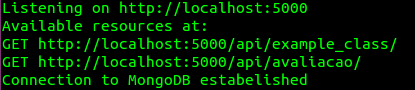
\includegraphics[scale=0.7]{imagens/outApiConsole.png}
    \end{center}
	\caption{\label{fig:api_console}Exemplo de servidor de API iniciado}
\end{figure}

O servidor \textit{Express} criado irá processar as \textit{requests} que forem recebidas, irá identificar a URI solicitada e o método HTTP e então irá encaminhar a \textit{request} para o \textit{router middleware} que, por sua vez, irá processar a \textit{request} e realizar a operação CRUD correspondente utilizando seu(s) respectivo(s) \textit{model(s)}. Esta sequência de processamento é mostrada no diagrama de sequências nas Figuras \ref{fig:seq_api_1} e \ref{fig:seq_api_2}.


\begin{figure}
    \begin{center}
        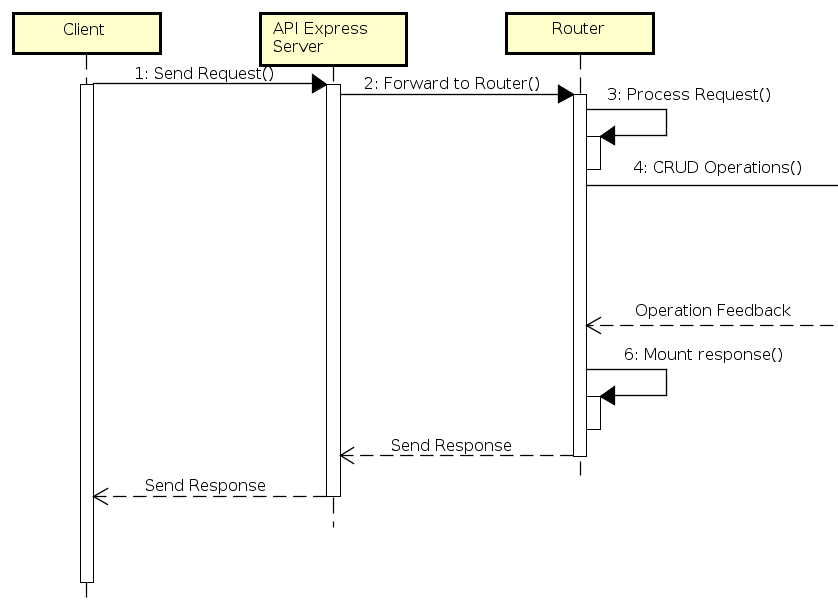
\includegraphics[scale=0.7]{imagens/API_Sequence_Diagram_1.png}
    \end{center}
	\caption{\label{fig:seq_api_1}Exemplo de processamento de \textit{request} no servidor da API - Parte 1}
\end{figure}

\begin{figure}
    \begin{center}
        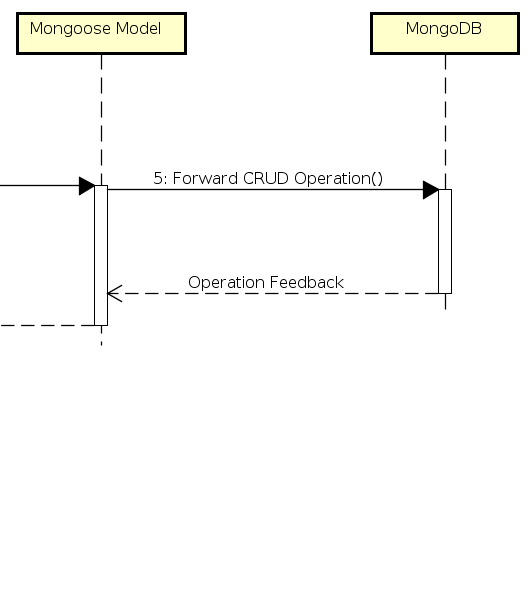
\includegraphics[scale=0.7]{imagens/API_Sequence_Diagram_2.png}
    \end{center}
	\caption{\label{fig:seq_api_2}Exemplo de processamento de \textit{request} no servidor da API - Parte 2}
\end{figure}


\chapter{Considerações Finais}
\label{chap:concl}

Neste trabalho, foi proposta uma solução para o problema de geração automática de APIs REST que provejam as funcionalidades necessárias para que sejam executadas as operações básicas de manutenção de documentos (CRUD - \textit{Create, Read, Update, Delete}), com o objetivo de utilizar a geração automática de código como uma forma de aumentar a confiabilidade e produtividade do processo de criação de software.

A solução AutoREST aplica os conceitos das metodologias de Engenharia de Software Baseada em Componentes, Desenvolvimento Dirigido por Modelos e Programação Generativa, concretizando heurísticas de cada uma destas metodologias em uma proposta de arquitetura de software. Além disto, propomos uma ferramenta como prova de conceito, que serve como instanciação desta arquitetura.

Este trabalho foi motivado pelo formalismo da arquitetura REST e a representatividade das notações JSON Schema e Diagrama de Classes UML. Através destas notações, foi possível a proposição de regras de modelagem que permitem a representação conceitual de uma API REST. Além disto, dada a estrutura da notação JSON Schema conforme \citeonline{PEZOA:2016}, que é baseada na Backus-Naur Form (BNF), foi possível a proposição de um método para a conversão da um documento JSON Schema em código fonte da API representada.

A arquitetura proposta, além dos componentes descritos para a instanciação desta arquitetura em uma prova de conceito, foram construídos a partir do estudo da arquitetura REST, do \textit{Hypertext Transfer Protocol} (HTTP) e das notações JSON Schema e UML, esta última particularmente no que concerne o conjunto da UML que é disponibilizado pela ferramenta Astah. Além destas tecnologias, foram estudadas a linguagem Node.js, o sistema gerenciador de bancos de dados MongoDB e o módulo Node.js Mongoose, que são utilizados pelas APIs REST geradas pela ferramenta proposta.

%------------------------------------------------------------

\section{Trabalhos Relacionados}
\label{sec:related}

Dentre os trabalhos encontrados que tratem de geração de código automática, foram selecionados alguns que tratam especificamente de ferramentas para a geração automática de código a partir de definições em formato JSON Schema ou similar. Se destacaram em nossa pesquisa as ferramentas Heroics, Schematic, Swagger e Eve. Além disso, damos destaque as ferramentas DaemonX e Prmd, que utilizam alterações na especificação de APIs para gerar a documentação e versionamento delas automaticamente.

%------------------------------------------------------------

\subsection{Heroics and Schematic}

Heroics é um gerador que utiliza um JSON Schema que representa uma API para gerar clientes HTTP em Ruby para esta API \cite{HEROICS}. Outro gerador que utiliza uma entrada similar, em JSON Hyper-Schema \cite{JSHYPERSCH}, para gerar clientes HTTP em Go é o Schematic \cite{SCHEMATIC}.

A principal diferença destas ferramentas para o AutoREST é o fato de gerarem apenas código cliente. Porém, o fato de utilizarem JSON Schema em seus processos pode significar que uma interação com elas seria algo que acrescentaria valor a solução AutoREST, permitindo assim que os clientes da API já fossem criados também de forma automática.

%------------------------------------------------------------

\subsection{Prmd}

Prmd \cite{PRMD} é uma ferramenta que permite realizar verificação e geração de documentação para APIs utilizando um JSON Schema que a descreve. O JSON Schema utilizado deve possuir algumas características descritas na documentação do Prmd.

Esta é outra ferramenta que utiliza o JSON Schema para um propósito diferente do AutoREST, pois gera documentação para uma API. Como as ferramentas anteriores, esta funcionalidade poderia ser alcançada com uma possível integração de um JSON Schema que descrevesse a REST API gerada.

%------------------------------------------------------------

\subsection{Swagger}

Swagger \cite{SWAGGER} é uma representação de REST APIs com um grande conjunto de ferramentas de apoio ao desenvolvimento e suporte, em várias das linguagens de programação atuais. Com uma definição Swagger, é possível a geração de documentação e geração de clientes. A especificação Swagger atualmente é gerenciada pela Open API Initiative (OAI) \cite{OpenAPII}.

As definições Swagger e o grande número de ferramentas de geração disponibilizadas pela comunidade proporcionariam o escopo restante no processo de criação de APIs que não é explorado no AutoREST. Uma especificação Swagger gerada pelo AutoREST poderia proporcionar tanto a criação de documentações quanto de códigos clientes da API.

%------------------------------------------------------------

\subsection{Eve}

Eve \cite{IAROCCI:EVE} é um \textit{framework} em Python para a disponibilização de REST APIs. É utilizada uma definição similar a JSON Schema que será interpretada e validada pela ferramenta Cerberus \cite{IAROCCI:CERBERUS}. Esta definição determina o \textit{schema} do \textit{resource} disponibilizado e os métodos HTTP disponíveis para o mesmo.

O \textit{framework} do Eve proporciona uma experiência com uma interação menos explícita com o sistema gerenciador de banco de dados, deixando para o desenvolvedor a tarefa de especificar na gramática da ferramenta Cerberus todos os seus \textit{resources} e artefatos relacionados.

A principal diferença para o AutoREST é que seria necessário criar um CM. Com este, a especificação dos \textit{resources} seria criada. Então, a API seria gerada e estaria pronta para ser utilizada.

%------------------------------------------------------------

\subsection{DaemonX}

DaemonX é uma plataforma extensível para o gerenciamento de evolução de documentos representativos de estruturas de dados. Dentre os usos desta plataforma está o de gerenciar a evolução de APIs REST com uma notação baseada no princípio de Arquiteturas Dirigidas por Modelos (MDA - \textit{Model-Driven Architecture}) \cite{POLAK:2015}.

Similar ao Prmd, esta aplicação da plataforma DaemonX apresenta uma forma de representar e gerenciar a evolução de APIs REST, uma funcionalidade não disponível na solução AutoREST. Entretanto, por utilizar uma representação específica, apesar de possivelmente atingir maior detalhamento das APIs, não seria de fácil integração com soluções mais gerais como a AutoREST.

%------------------------------------------------------------

\section{Conclusão}

Nesta seção, são apresentadas respostas para as perguntas de pesquisa propostas no início deste documento utilizando a experiência obtida durante o desenvolvimento deste trabalho e implementação da ferramenta prova de conceito.

\begin{itemize}
	\item QP1. Existe viabilidade na automação da geração de uma API REST utilizando uma abordagem baseada em MDD?
\end{itemize}

Esta automação é viável, desde que sejam compreendidos seus pontos positivos e negativos, que no decorrer deste trabalho podemos assumir como sendo:

\begin{itemize}
	\item \textbf{Positivos}
	\begin{itemize}
		\item Para APIs não customizadas após a geração, o modelo é altamente representativo do código fonte e o custo de evolução e manutenção é baixo
		\item Fácil transição de conhecimento sobre o funcionamento da API sem a necessidade de olhar código fonte e outras estruturas de baixo nível
	\end{itemize}
	\item \textbf{Contras}
	\begin{itemize}
		\item APIs customizadas tem seu código customizado perdido no momento de uma nova geração a partir do modelo
		\item É necessária uma boa compreenção das regras de modelagem a serem utilizadas
	\end{itemize}
\end{itemize}

\begin{itemize}
	\item QP2. Quais os elementos necessários para a representação completa de uma API REST em um modelo gráfico para que este possa ser utilizado como modelo de configuração em uma abordagem MDD para a geração de uma API com todas as funcionalidades CRUD fundamentais?
\end{itemize}

Como mencionado na Seção \ref{sec:cmr}, alguns elementos se mostraram essenciais para a representação de uma API REST. Em particular, a necessidade de representar todas as entidades com identificadores únicos se mostrou importante para a modelagem apropriada das APIs; reconhecer a restrição da arquitetura REST de como são definidos endpoints deve reger a escolha de modelos de representação e elementos utilizados nestes. A representação de associações deve ser suficientemente clara para que os endpoints gerados possam ser identificados corretamente. Pela experiência obtida durante o desenvolvimento da prova de conceito, não é recomendado o uso de chaves compostas para identificação de recursos.

\begin{itemize}
	\item QP3. Existe a necessidade de criação de um modelo intermediário, a partir de um modelo de configuração, que sirva como artefato de entrada para um gerador de APIs REST?
\end{itemize}

Existe se o modelo de configuração for muito abstrato e o gerador de APIs não compreender o mesmo nível de abstração. No caso da solução apresentada neste trabalho, tomou-se a decisão de usar um modelo intermediário que possibilitasse uma validação sintática automática e uma leitura humana e computacional rápida. Acreditamos que se usado apenas um modelo gráfico, com definição semântica ampla, não teria um resultado de mesma qualidade.

\begin{itemize}
	\item QP4. As APIs REST são suficientemente modularizáveis a ponto de permitir a geração automática de código a partir de blocos de código parametrizáveis? Qual a complexidade de se criar um compilador de APIs REST que não se utiliza de uma abordagem GP?
\end{itemize}

Considerando que a API gerada pela solução apresentada neste trabalho é em Node.js, foi obtida boa utilização dos blocos de código parametrizáveis (\textit{snippets}). O fato da arquitetura REST impor a divisão em camadas e reforçar o uso de um formato de \textit{resource} no sistema contribuiu para esta modularização. Sem a abordagem GP, acreditamos que a implementação poderia ficar maior e mais difícil de manter, pois a necessidade de atualizar um \textit{snippet} geraria trabalho manual.

\begin{itemize}
	\item QP5. É possível a geração automática de um banco de dados auxiliar à API REST?
\end{itemize}

O trabalho nos leva a concluir que sim, é possivel gerar um banco de dados auxiliar a uma API REST. Algumas incompatibilidades entre a especificação MDD e o banco de dados podem atrapalhar esta geração. Neste trabalho, estas incompatibilidades foram endereçadas, gerando uma API mais robusta e utilizando algumas funções do banco de dados de uma forma semântica específica. Por exemplo, a relação de herança entre \textit{resources} foi tratada adicionando um atributo oculto de tipo (\textit{\_\_type}) e armazenando todas as classes filhas na mesma coleção da classe pai. Acreditamos que este seja um exemplo de boa utilização dos recursos de um sistema de gerência de banco de dados para a implementação de características da arquitetura REST.

\begin{itemize}
	\item QP6. Diagramas de Classes UML são uma notação adequada para a modelagem de APIs REST?
\end{itemize}

Muitos fatores podem influenciar a resposta para esta pergunta. Um dos mais importante deles seria a respeito do tipo de banco de dados utilizado. Se o banco de dados for relacional, então algumas definições de dados serão levemente alteradas. Porém, as restrições de relacionamento entre os \textit{resources} serão melhor reforçadas. No caso de um banco de dados não-relacional, as restrições de relacionamento podem ficar um pouco mais livres, podendo levar a referências inválidas. Entretanto, as definições dos dados podem ser mais fiéis ao diagrama de classes.

\begin{itemize}
	\item QP7. Arquivos JSON Schema são adequados para a representação de APIs REST?
\end{itemize}

Acreditamos que a especificação JSON Schema, na forma restritiva especificada por \citeonline{PEZOA:2016}, seja insuficiente para a representação fiél de uma RESTful API. Apesar de ser um formato de dados que é utilizado na maioria das transações web e a geração de um JSON Schema ser algo de grande valor, as características do sistema requerem determinadas restrições e definições que não estão disponíveis em JSON Schema.

\begin{itemize}
	\item QP8. O SGBD MongoDB, a linguagem Node.js e a biblioteca Mongoose são adequadas como tecnologias para a geração automática de APIs REST?
\end{itemize}



%------------------------------------------------------------

\section{Trabalhos Futuros}

Diversos trabalhos podem ser realizados expandindo o tema deste estudo. Nesta seção, definimos alguns temas que surgiram ao longo da realização do estudo, mas que por estar além do escopo proposto ou requirir um dispêndio de tempo não disponível, não foram explorados.

\begin{itemize}
    \item A ferramenta Astah é extensível através do uso de \textit{plugins}. A implementação de um \textit{plugin} Astah para a geração de modelos de configuração segundo as especificações deste trabalho seria de grande ajuda na modelagem de APIs REST e execução de ferramentas AutoREST. Dentre os requisitos que este \textit{plugin} deverá cumprir estão a criação automática de \textit{tags} conforme as especificações da Seção \ref{sec:xmi}, a limitação dos tipos de atributos disponíveis, a limitação dos tipos de associação disponíveis e uma interface de ajuda que apresente as regras listadas na Seção \ref{sec:xmi} para fácil acesso a referência.

    \item Algumas das ferramentas listadas na Seção \ref{sec:related} permitem: a geração automática de código para funcionalidades diferentes das propostas pela solução AutoREST, e; o gerenciamento da documentação e versionamento de APIs REST. Visto que algumas destas ferramentas utilizam especificações em notações derivadas de JSON, seria útil a adequação das especificações destas diversas ferramentas e a integração de seus ambientes para execução em conjunto.

    \item Devido a limitações da ferramenta Astah, determinados tipos de associação disponíveis na UML não puderam ser definidos para modelagem neste estudo. A definição de regras para a modelagem e conversão destes tipos de associação seria útil para aumentar a versatilidade da solução proposta. Dentre estas associações, se destacam: as associações de Generalização/Especialização para representar o conceito de herança múltipla; o uso dos esteriótipos \textit{Disjoint} e \textit{Overlapping} para associações de Generalização/Especialização, e; a definição de navegabilidade em associações de agregação.

    \item A modelagem e implementação da ferramenta usada como prova de conceito da arquitetura proposta está limitada as tecnologias determinadas em sua especificação. A criação de outras possíveis implementações da arquitetura AutoREST serviria para validar a sua proposta de independência de tecnologia; além disto, acreditamos que possam haver tecnologias de modelagem mais apropriadas para a definição de uma API REST, permitindo a geração não só de operações CRUD mas de outras funcionalidades mais especializadas. Tecnologias que poderiam ser utilizadas para diferentes implementações são: para modelos de configuração, Diagramas de Classes UML gerados por ferramentas diferentes do Astah, ou Modelos Entidade-Relacionais; para PFIS, estruturas em linguagem RAML, Swagger ou WSDL, e; para geração de código, linguagens como ASP.NET ou php.
\end{itemize}


% ----------------------------------------------------------

% ---
% Finaliza a parte no bookmark do PDF
% para que se inicie o bookmark na raiz
% e adiciona espaço de parte no Sumário
% ---
\phantompart

% ----------------------------------------------------------
% ELEMENTOS PÓS-TEXTUAIS
% ----------------------------------------------------------
\postextual

% ----------------------------------------------------------
% Referências bibliográficas
% ----------------------------------------------------------

%------------------------- AQUI VAI O BIBSTYLE
%\bibliographystyle{alpha}
%---------------------------------------------

\bibliography{basic.bib}

% ----------------------------------------------------------
% Glossário
% Consulte o manual da classe abntex2 para orientações sobre o glossário.
%\glossary

% ----------------------------------------------------------
% Apêndices
% ---
% Inicia os apêndices
% ---
%\begin{apendicesenv}
% Imprime uma página indicando o início dos apêndices
%\partapendices
%\chapter{Quisque libero justo}
%\lipsum[50]
%\end{apendicesenv}
% ----------------------------------------------------------

% Anexos
% ---
% Inicia os anexos
% ---
%\begin{anexosenv}
% Imprime uma página indicando o início dos anexos
%\partanexos
%\chapter{Morbi ultrices rutrum lorem.}
%\lipsum[30]
%\end{anexosenv}

\begin{anexosenv}
\partanexos
\chapter{Lista de \textit{Status Codes}}
\label{anexo:status}
\begin{table}[H]
    \centering
    \begin{tabular}{|l|l|}
    \hline
    \textit{Code} & \textit{Reason-Phrase}                 \\
    \hline
    100  & Continue                      \\
    101  & Switching Protocols           \\
    200  & OK                            \\
    201  & Created                       \\
    202  & Accepted                      \\
    203  & Non-Authoritative Information \\
    204  & No Content                    \\
    205  & Reset Content                 \\
    206  & Partial Content               \\
    300  & Multiple Choices              \\
    301  & Moved Permanently             \\
    302  & Found                         \\
    303  & See Other                     \\
    304  & Not Modified                  \\
    305  & Use Proxy                     \\
    307  & Temporary Redirect            \\
    400  & Bad Request                   \\
    401  & Unauthorized                  \\
    402  & Payment Required              \\
    403  & Forbidden                     \\
    404  & Not Found                     \\
    405  & Method Not Allowed            \\
    406  & Not Acceptable                \\
    407  & Proxy Authentication Required \\
    408  & Request Timeout               \\
    409  & Conflict                      \\
    410  & Gone                          \\
    411  & Length Required               \\
    412  & Precondition Failed           \\
    413  & Payload Too Large             \\
    414  & URI Too Long                  \\
    415  & Unsupported Media Type        \\
    416  & Range Not Satisfiable         \\
    417  & Expectation Failed            \\
    426  & Upgrade Required              \\
    500  & Internal Server Error         \\
    501  & Not Implemented               \\
    502  & Bad Gateway                   \\
    503  & Service Unavailable           \\
    504  & Gateway Timeout               \\
    505  & HTTP Version Not Supported    \\
    \hline
    \end{tabular}
\end{table}

\chapter{Gramática BNF de JSON Schema}
\label{anexo:bnfjs}
Gramática BNF conforme \citeonline{CSWR:GRAMMAR}.

\begin{lstlisting}
JSDoc := { ( id, )? ( defs, )? JSch }
id := "id": "uri"
defs := "definitions": { kSch (, kSch)*}
kSch := kword: { JSch }
JSch := ( res (, res)*)
res := type | strRes | numRes | arrRes | objRes | multRes
     | refSch | title | description
type := "type" : ([typename (, typename)*] | typename)
typename := "string" | "integer" | "number" | "boolean" | "null"
          | "array" | "object"
title := "title":  string
description := "description":  string
strRes :=  minLen | maxLen | pattern
minLen := "minLength": n
maxLen := "maxLength": n
pattern := "pattern": "regExp"
numRes := min | max | multiple 
min := "minimum": r (,exMin)?
exMin := "exclusiveMinimum": bool
max := "maximum": r (,exMax)?
exMax := "exclusiveMaximum": bool
multiple := "multipleOf": r   (r >= 0)
arrRes := items | additems | minitems | maxitems  | unique
items := ( sameitems |  varitems )
sameitems := "items": { JSch }
varitems := "items": [{ JSch }(,{ JSch })*] 
additems :=  "additionalItems": (bool | { JSch })
minitems := "minItems": n
maxitems := "maxItems": n
unique := "uniqueItems": bool
objRes := prop | addprop | req | minprop | maxprop | dep | pattprop
prop := "properties": { kSch (, kSch)*}
kSch := kword: { JSch }
addprop := "additionalProperties": (bool | { JSch })
req := "required": [ kword (, kword)*]
minprop := "minProperties": n
maxprop := "maxProperties": n
dep := "dependencies": { kDep (, kDep)*}
kDep := (kArr | kSch)
kArr := kword: [ kword (, kword)*]
pattprop := "patternProperties": { patSch (, patSch)*}
patSch := "regExp": { JSch }
multRes := allOf | anyOf| oneOf | not | enum
anyOf := "anyOf": [ { JSch } (, { JSch }) * ]
allOf := "allOf": [ { JSch } (, { JSch }) * ]
oneOf := "oneOf": [ { JSch } (, { JSch }) * ]
not := "not": { JSch }
enum := "enum": [Jval (, Jval)*]
refSch := "\$ref": "uriRef" 
uriRef := ( address )? ( \# / JPointer )?
JPointer := ( / path )
path := ( unescaped | escaped )
escaped := ~0 | ~1
address = (scheme : )? hier-part (? query )

\end{lstlisting}

%-----------------------------------------

\chapter{JSON Schema relativo a Figura \ref{fig_example_class}}
\label{fig_example_class_j}

\begin{listing}
\begin{minted}[frame=single,
               framesep=3mm,
               linenos=true,
               xleftmargin=21pt,
               tabsize=4]{js}
{     
    "definitions": {
        "Example_Class": {
            "type": "object",
            "additionalProperties": false,
            "properties": {
                "attribute0": {
                    "type": "integer"
                },
                "attribute1": {
                    "type": "boolean"
                },
                "attribute2": {
                    "type": "integer",
                    "minimum": 0,
                    "maximum": 255
                },
                "attribute3": {
                    "type": "string",
                    "maxLength": 1
                },
                "attribute4": {
                    "type": "number"
                },
                "attribute5": {
                    "type": "number"
                },
                "attribute6": {
                    "type": "integer"
                },
                ...
            }
        }
    }
}
\end{minted}
\caption{JSON Schema criado a partir da Figura \ref{fig_example_class} - Parte 1}
\end{listing}

\begin{listing}
\begin{minted}[frame=single,
               framesep=3mm,
               linenos=true,
               xleftmargin=21pt,
               breaklines=true,
               tabsize=4]{js}
{
    {
        {
            {
                ...
                "attribute7": {
                    "type": "integer"
                },
                "attribute8": {
                    "type": "array"
                    "items":{
                        "type": "integer"
                    }
                },
                "attribute9": {
                    "type": "string",
                    "format": "date-time"
                },
                "attribute10": {
                    "type": "object"
                },
                "attribute11": {
                    "type": "string",
                    "minLength": 3,
                    "maxLength": 140,
                    "pattern": "/^[a-zA-Z]*$/"
                }
            },
            "dependencies": {
                "attribute1": [ "attribute0" ],
                "attribute2": [ "attribute0" ],
                "attribute3": [ "attribute0" ],
                "attribute4": [ "attribute0" ],
                "attribute5": [ "attribute0" ],
                "attribute6": [ "attribute0" ],
                "attribute7": [ "attribute0" ],
                "attribute8": [ "attribute0" ],
                "attribute9": [ "attribute0" ],
                "attribute10": [ "attribute0" ],
                "attribute11": [ "attribute0" ]
            }
            "required": {
                [ "attribute0", "attribute1", "attribute3", "attribute4", "attribute5", "attribute6", "attribute7", "attribute8", "attribute9", "attribute10", "attribute11" ]
            }
        }
    }
}
\end{minted}
\caption{JSON Schema criado a partir da Figura \ref{fig_example_class} - Parte 2}
\end{listing}

%-----------------------------------------

\chapter{JSON Schema relativo a Figura \ref{fig_example_multiplicity}}
\label{fig_example_multiplicity_j}

\begin{listing}
\begin{minted}[frame=single,
               framesep=3mm,
               linenos=true,
               xleftmargin=21pt,
               breaklines=true,
               tabsize=4]{js}
{
    "definitions": {
        "Class0": {
            "type": "object",
            "additionalProperties": false,
            "properties": {
                "attribute0": {
                    "type": "integer"
                },
                "attribute1": {
                    "type": "integer"
                },
                "Class1_created_identifier": {
                    "type": "integer"
                },
                "Class2_attribute3": {
                    "type": "array",
                    "items": {
                        "type": "integer"
                    }
                }
            },
            "dependencies": {
                "attribute1": [ "attribute0" ],
                "Class1_created_identifier": [ "attribute0" ],
                "Class2_attribute3": [ "attribute0" ]
            },
            "required": { 
                [ "attribute0" ]
            }
        },
        ...
    }
}
\end{minted}
\caption{JSON Schema criado a partir da Figura \ref{fig_example_multiplicity} - Parte 1}
\end{listing}

\begin{listing}
\begin{minted}[frame=single,
               framesep=3mm,
               linenos=true,
               xleftmargin=21pt,
               breaklines=true,
               tabsize=4]{js}
{    
    {
        ...,
        "Class1": {
            "type": "object",
            "additionalProperties": false,
            "properties": {
                "created_identifier": {
                    "type": "integer"
                },
                "attribute2": {
                    "type": "integer"
                },
                "Class0_attribute0": {
                    "type": "integer"
                },
                "Class3_attribute4": {
                    "type": "integer"
                }
            },
            "dependencies": {
                "attribute2": [ "created_identifier" ],
                "Class0_attribute0": [ "created_identifier" ],
                "Class3_attribute4": [ "created_identifier" ]
            },
            "required": {
                [ "created_identifier", "attribute0" ]
            }
        },
        ...
    }
}
\end{minted}
\caption{JSON Schema criado a partir da Figura \ref{fig_example_multiplicity} - Parte 2}
\end{listing}

\begin{listing}
\begin{minted}[frame=single,
               framesep=3mm,
               linenos=true,
               xleftmargin=21pt,
               breaklines=true,
               tabsize=4]{js}
{
    {
        ...,
        "Class2": {
            "type": "object",
            "additionalProperties": false,
            "properties": {
                "attribute3": {
                    "type": "integer"
                },
                "Class0_attribute0": {
                    "type": "array",
                    "items": {
                        "type": "integer"
                    }
                },
                "Class3_attribute4": {
                    "type": "array",
                    "items": {
                        "type": "integer"
                    }
                    "minLength": 1
                }
            },
            "dependencies": {
                "Class0_attribute0": [ "attribute3" ],
                "Class3_attribute4": [ "attribute3" ]
            },
            "required": {
                [ "attribute3", "attribute4" ]
            }
        },
        ...
    }
}
\end{minted}
\caption{JSON Schema criado a partir da Figura \ref{fig_example_multiplicity} - Parte 3}
\end{listing}

\begin{listing}
\begin{minted}[frame=single,
               framesep=3mm,
               linenos=true,
               xleftmargin=21pt,
               breaklines=true,
               tabsize=4]{js}
{
    {
        ...,
        "Class3": {
            "type": "object",
            "additionalProperties": false,
            "properties": {
                "attribute4": {
                    "type": "integer"
                }
            },
            "dependencies": {
            
            },
            "required": {
                [ "attribute4" ]
            }
        }
    }
}
\end{minted}
\caption{JSON Schema criado a partir da Figura \ref{fig_example_multiplicity} - Parte 4}
\end{listing}

%-----------------------------------------

\chapter{JSON Schema relativo a Figura \ref{fig_example_realization}}
\label{fig_example_realization_j}

\begin{listing}
\begin{minted}[frame=single,
               framesep=3mm,
               linenos=true,
               xleftmargin=21pt,
               breaklines=true,
               tabsize=4]{js}
{
    "definitions": {
        "Class4": {
            "type": "object",
            "additionalProperties": false,
            "properties": {
                "attribute5": {
                    "type": "integer"
                }
            },
            "dependencies": {
            
            },
            "required": {
                [ "attribute5" ]
            }
        },
        ...,
    }
}
\end{minted}
\caption{JSON Schema criado a partir da Figura \ref{fig_example_realization} - Parte 1}
\end{listing}

\begin{listing}
\begin{minted}[frame=single,
               framesep=3mm,
               linenos=true,
               xleftmargin=21pt,
               breaklines=true,
               tabsize=4]{js}
{
    {
        ...,
        "Class5": {
            "type": "object",
            "additionalProperties": false,
            "properties": {
                "Class4_Inherited": {
                    "\$ref": "#/definitions/Class4"
                },
                "attribute7": {
                    "type": "integer"
                }
            },
            "dependencies": {
            
            },
            "required": {
                
            }
        }, 
        "Class8": {
            "type": "object",
            "additionalProperties": false,
            "properties": {
                "Class4_Inherited": {
                    "\$ref": "#/definitions/Class4"
                },
                "attribute6": {
                    "type": "integer"
                }
            },
            "dependencies": {
            
            },
            "required": {
                
            }
        },
        ...,
    }
}
\end{minted}
\caption{JSON Schema criado a partir da Figura \ref{fig_example_realization} - Parte 2}
\end{listing}

\begin{listing}
\begin{minted}[frame=single,
               framesep=3mm,
               linenos=true,
               xleftmargin=21pt,
               breaklines=true,
               tabsize=4]{js}
{
    {
        ...,
        "Class6": {
            "type": "object",
            "additionalProperties": false,
            "properties": {
                "Class5_Inherited": {
                    "\$ref": "#/definitions/Class4"
                },
                "attribute9": {
                    "type": "integer"
                }
            },
            "dependencies": {
            
            },
            "required": {
                
            }
        },
        
        "Class7": {
            "type": "object",
            "additionalProperties": false,
            "properties": {
                "Class5_Inherited": {
                    "\$ref": "#/definitions/Class4"
                },
                "attribute8": {
                    "type": "integer"
                }
            },
            "dependencies": {
            
            },
            "required": {
                
            }
        }
    }
}              
\end{minted}
\caption{JSON Schema criado a partir da Figura \ref{fig_example_realization} - Parte 3}
\end{listing}

%-----------------------------------------

\chapter{JSON Schema relativo a Figura \ref{fig_example_aggregation}}
\label{fig_example_aggregation_j}

\begin{listing}
\begin{minted}[frame=single,
               framesep=3mm,
               linenos=true,
               xleftmargin=21pt,
               breaklines=true,
               tabsize=4]{js}
{
    "definitions": {
        "Class10": {
            "type": "object",
            "additionalProperties": false,
            "properties": {
                "attribute2": {
                    "type": "integer"
                },
                "Class11_attribute1": {
                    "type": "array",
                    "items": {
                        "type": "integer"
                    }
                },
                "Class12_attribute3": {
                    "type": "array",
                    "items": {
                        "type": "integer"
                    }
                }
            },
            "dependencies": {
                "Class11_attribute1": [ "attribute2" ],
                "Class12_attribute3": [ "attribute2" ]
            },
            "required": {
                [ "attribute2" ]
            }
        },
        ...
    }
}
\end{minted}
\caption{JSON Schema criado a partir da Figura \ref{fig_example_aggregation} - Parte 1}
\end{listing}


\begin{listing}
\begin{minted}[frame=single,
               framesep=3mm,
               linenos=true,
               xleftmargin=21pt,
               breaklines=true,
               tabsize=4]{js}
{
    {
        ...,
        "Class11": {
            "type": "object",
            "additionalProperties": false,
            "properties": {
                "attribute1": {
                    "type": "integer"
                },
                "Class9": {
                    "type": "object",
                    "additionalProperties": false,
                    "properties": {
                        "attribute0": {
                            "type": "integer"
                        }
                    },
                    "dependencies": {
                    
                    },
                    "required": {
                        [ "attribute0" ]
                    }
                }
            },
            "dependencies": {
                "Class9": [ "attribute1" ]
            },
            "required": {
                [ "attribute1" ]
            }
        },
        ...
    }
}
\end{minted}
\caption{JSON Schema criado a partir da Figura \ref{fig_example_aggregation} - Parte 2}
\end{listing}

\begin{listing}
\begin{minted}[frame=single,
               framesep=3mm,
               linenos=true,
               xleftmargin=21pt,
               breaklines=true,
               tabsize=4]{js}
{
    {
        ...,
        "Class12": {
            "type": "object",
            "additionalProperties": false,
            "properties": {
                "attribute3": {
                    "type": "integer"
                },
                "Class10_Refs": {
                    "type": "array",
                    "items": {
                        "\$ref": "#/definitions/Class10"
                    },
                    "minLength": 1
                }
            },
            "dependencies": {
                "Class10_Refs": [ "attribute3" ]
            },
            "required": {
                [ "attribute3" ]
            }
        }
    }
}
\end{minted}
\caption{JSON Schema criado a partir da Figura \ref{fig_example_aggregation} - Parte 3}
\end{listing}

%-----------------------------------------

\chapter{JSON Schema relativo a Figura \ref{fig_example_association_class}}
\label{fig_example_association_class_j}

\begin{listing}
\begin{minted}[frame=single,
               framesep=3mm,
               linenos=true,
               xleftmargin=21pt,
               breaklines=true,
               tabsize=4]{js}
{
    "definitions": {
        "AssociationClass0": {
            "type": "object",
            "additionalProperties": false,
            "properties": {
                "Class13_attribute0": {
                    "type": "integer"
                },
                "Class14_attribute1": {
                    "type": "integer"
                },
                "attribute2": {
                    "type": "integer"
                },
                "attribute3": {
                    "type": "integer"
                }
            },
            "dependencies": {
                "attribute2": [ "Class13_attribute0", "Class14_attribute1" ],
                "attribute3": [ "Class13_attribute0", "Class14_attribute1" ],
                "Class13_attribute0": [ "Class14_attribute1" ],
                "Class14_attribute1": [ "Class13_attribute0" ]
            },
            "required": {
                [ "Class13_attribute0", "Class14_attribute1" ]
            }
        },
        ...
    }
}
\end{minted}
\caption{JSON Schema criado a partir da Figura \ref{fig_example_association_class} - Parte 1}
\end{listing}

\begin{listing}
\begin{minted}[frame=single,
               framesep=3mm,
               linenos=true,
               xleftmargin=21pt,
               breaklines=true,
               tabsize=4]{js}
{
    {
        ...,
        "Class13": {
            "type": "object",
            "additionalProperties": false,
            "properties": {
                "attribute0": {
                    "type": "integer"
                },
                "AssociationClass0_Link": {
                    "type": "array",
                    "items": {
                        "type": "object",
                        "properties": {
                            "\$ref": "#/definitions/AssociationClass0"
                        }
                    }
                }
            },
            "dependencies": {
                "AssociationClass0_Link": [ "attribute0" ]
            },
            "required": {
                [ "attribute0" ]
            }
        },
        ...
    }
}
\end{minted}
\caption{JSON Schema criado a partir da Figura \ref{fig_example_association_class} - Parte 2}
\end{listing}

\begin{listing}
\begin{minted}[frame=single,
               framesep=3mm,
               linenos=true,
               xleftmargin=21pt,
               breaklines=true,
               tabsize=4]{js}
{
    {
        ...,
        "Class14": {
            "type": "object",
            "additionalProperties": false,
            "properties": {
                "attribute1": {
                    "type": "integer"
                },
                "AssociationClass0_Link": {
                    "type": "array",
                    "items": {
                        "type": "object",
                        "properties": {
                            "\$ref": "#/definitions/AssociationClass0"
                        }
                    }
                }
            },
            "dependencies": {
                "AssociationClass0_Link": [ "attribute1" ]
            },
            "required": {
                [ "attribute1" ]
            }
        }
    }
}
\end{minted}
\caption{JSON Schema criado a partir da Figura \ref{fig_example_association_class} - Parte 3}
\end{listing}

%-----------------------------------------

\chapter{Model Mongoose para a classe da Figura \ref{fig_example_class}}
\label{anexo:model_mongoose}

\begin{listing}

\begin{minted}[frame=single,
               framesep=3mm,
               linenos=true,
               xleftmargin=21pt,
               breaklines=true,
               tabsize=4]{js}
var mongoose = require('mongoose'),
    integerValidator = require('mongoose-integer'),
    Schema = mongoose.Schema;

var Example_ClassSchema = new Schema({
    _id: {
        type: Number,
        integer: true,
        required: true,
        unique: true
    },
    attribute1: {
        type: Boolean,  required: true
    },
    attribute2: {
        type: Number,
        integer: true,
        minimum: 0,
        maximum: 255
    },
    attribute3: {
        type: String,   maxlength: 1,   required: true
    },
    attribute4: {
        type: Number,   required: true
    },
    attribute5: {
        type: Number,   required: true
    },
    attribute6: {
        type: Number,
        integer: true,
        required: true
    },
    ...
}
\end{minted}
%\caption{Model Mongoose - Parte 1}
\end{listing}

\begin{listing}
\begin{minted}[frame=single,
               framesep=3mm,
               linenos=true,
               xleftmargin=21pt,
               breaklines=true,
               tabsize=4]{js}
{
    ...
    attribute7: {
        type: Number,
        integer: true,
        required: true
    },
    attribute8: {
        any: [{ type: Number,   integer: true   }]
    },
    attribute9: {
        type: Date,
        required: true
    },
    attribute10: {
        type: Object,   required: true
    },
    attribute11: {
        type: String,
        minlength: 3,
        maxlength: 140,
        match: /^[a-zA-Z]*$/,
        required: true
    }
});

Example_ClassSchema.virtual('attribute0').get(function() {
    return this._id;
});
Example_ClassSchema.virtual('attribute0').set(function (value) {
    this._id = value;
});

Example_ClassSchema.plugin(integerValidator);

Example_ClassSchema.methods.cleanObject = function() {
    var doc = this.toObject({ virtuals: true });
    delete doc.__v;
    delete doc._id;
    delete doc.id;
    return doc;
};

module.exports = mongoose.model('Example_Class', Example_ClassSchema);

\end{minted}
\caption{Model Mongoose - Parte 2}
\end{listing}

\end{anexosenv}

%---------------------------------------------------------------------
% INDICE REMISSIVO
%---------------------------------------------------------------------
\phantompart
\printindex
\end{document}
